\documentclass{icsc2017a}
\graphicspath{{fig/}}

\usepackage[
    font=footnotesize,
    labelfont=bf
]{caption}
\usepackage{siunitx}
\usepackage{algorithm,algpseudocode}
\usepackage{pgfplots}
\usepackage[font=scriptsize]{subcaption}

% give algorithms a refname or else just a number is displayed with autoref
\newcommand{\algorithmautorefname}{Algorithm}
% make section start with a capital S
\renewcommand{\sectionautorefname}{Section}

\pgfplotsset{
    compat=1.14,
    every tick label/.append style={font=\tiny},
    every axis/.append style={
        font=\scriptsize,
        xtick pos=left % remove x ticks from top of figure
    },
    every axis x label/.append style = {
        at={(ticklabel cs:0.5,-2)},
        anchor=center
    },
    every axis y label/.append style = {
        at={(ticklabel cs:0.5,-2)},
        anchor=center
    },
    legend columns=2,
    legend style={font=\tiny}
}

% define my url command
\newcommand{\myurl}[1]{\href{#1}{#1}}

% define common math terms
\newcommand{\mass}{\bm{M}}
\newcommand{\damping}{v \bm{C}_1}
\newcommand{\stiffness}{g \bm{K}_0 + v^2 \bm{K}_2}

% state terms
\newcommand{\dstate}{\dot{\bm{x}}}
\newcommand{\state}{\bm{x}}
\newcommand{\sysInput}{\bm{u}}
\newcommand{\sysOutput}{y}
\newcommand{\stateMat}{\bm{A}}
\newcommand{\inputMat}{\bm{B}}
\newcommand{\outputMat}{\bm{C}}

% estimate terms
\newcommand{\dstateEst}{\dot{\hat{\bm{x}}}}
\newcommand{\stateEst}{\hat{\bm{x}}}
\newcommand{\meas}{z}
\newcommand{\processCov}{\bm{Q}}
\newcommand{\processNoise}{\bm{w}}
\newcommand{\measCov}{R}
\newcommand{\measNoise}{v}
\newcommand{\kalmanGain}{\bm{K}}
\newcommand{\estimateCov}{\bm{P}}

% coordinates and speeds
\newcommand{\x}{x_{p}}
\newcommand{\y}{y_{p}}
\newcommand{\pitch}{\theta}
\newcommand{\yaw}{\psi}
\newcommand{\roll}{\phi}
\newcommand{\steer}{\delta}
\newcommand{\dx}{\dot{x}_{p}}
\newcommand{\dy}{\dot{y}_{p}}
\newcommand{\pitchRate}{\dot{\theta}}
\newcommand{\yawRate}{\dot{\psi}}
\newcommand{\rollRate}{\dot{\phi}}
\newcommand{\steerRate}{\dot{\delta}}
\newcommand{\rollAccel}{\ddot{\phi}}
\newcommand{\steerAccel}{\ddot{\delta}}

% pre/post
\newcommand{\pre}{-}
\newcommand{\post}{+}

% virtual/physical
\newcommand{\virtual}{\rho}
\newcommand{\physical}{\pi}

\begin{document}
\begin{flushleft}
{\fontsize{16pt}{20pt}\selectfont
    Description of a model based bicycle simulator}
\end{flushleft}
\begin{flushleft}
  {\fontsize{12}{14}{O. Lee, G. Dialynas, J. C. F. de Winter, R. Happee, A. L. Schwab}\\}
  \textit{Department of BioMechanical Engineering\\
    Delft University of Technology\\
    Mekelweg 2, 2628 CD Delft, The Netherlands\\
    e-mail: \{o.z.lee, g.dialynas, j.c.f.dewinter, r.happee, a.l.schwab\}@tudelft.nl}
\end{flushleft}
\section{Introduction}
Recent years have seen an increase in cycling as a transport mode in urban centers.
This has spurred an interest in the use of bicycle simulators to study cyclist behavior \cite{caro2015role,
herpers2008fivis, ohern2017validation, plumert2004childrens}.
However, few implement a model based approach that couples the bicycle roll and steer in a
realistic manner \cite{yin2007implementation}.
Balancing is a key task in cycling and we aimed to develop a simulator that allows us to study the effect of balance on
the rider's higher level cognitive decisions.

\section{Bicycle model and state estimation}
\label{sec:model_and_estimator}
The simulator implements the Whipple bicycle model using the benchmark parameters \cite{meijaard2007linearized}, as it is
a simple model that has been experimentally verified \cite{kooijman2008experimental}.
The Whipple model uses linearized equations of motion to describe the bicycle stability in terms of roll angle $\roll$ and
steer angle $\steer$.
These equations can be expressed in state space form parameterized by forward speed $v$
\begin{equation}
    \dstate = \stateMat{(v)} \state + \inputMat \sysInput \label{eq:state_space}
\end{equation}
where $ \dstate = \begin{bmatrix} \yawRate & \rollRate & \steerRate & \rollAccel & \steerAccel \end{bmatrix}^T $,
$ \state = \begin{bmatrix} \yaw & \roll & \steer& \rollRate & \steerRate \end{bmatrix}^T $,
$ \sysInput = \begin{bmatrix} T_\roll & T_\steer  \end{bmatrix}^T $, and expressions for $ \stateMat(v) $ and
$ \inputMat $ can be obtained from \cite{meijaard2007linearized}.
Note that our formulation extends the state by adding yaw angle $ \yaw $ because yaw rate $ \yawRate $ can be expressed linearly in terms of the state $\state$.
While roll torque $ T_\roll $ is an input to the system, it is not measured and cannot be applied by the
rider in our simulator since experiments have shown steer control to be the dominant rider control
action \cite{moore2011rider}.
Because the simulator has a fixed base, $\roll$ and $\yaw$ do not physically exist and cannot be measured
with sensors.
We treat them as unmeasured states and a Kalman filter is used to obtain an estimate.

\section{Simulator description}
An image of the fixed base simulator is shown in \autoref{fig:mech}. The physical system consists of a steering shaft,
the rear half of a bicycle frame, and rollers.
Reach and stack can be adjusted for a given rider as the steering shaft is telescopic and connected to the frame using
prismatic joints.
The steering shaft incorporates a high resolution angular encoder, an inline torque sensor, and an
electric motor connected in a direct drive configuration.
A lower resolution angular encoder measures rear wheel position and is used to estimate $v$.

The simulation of the bicycle model and state estimator are implemented in a microcontroller that runs an update loop at
a rate of \SI{1}{\kilo\hertz}.
Because the bicycle itself is visualized in our simulator, and the expressions for the rear wheel position coordinates
$\x$, $\y$ are nonlinear, explicit integration is used to obtain an extended state
$\bm{x}_e = \begin{bmatrix} \x & \y & \yaw & \roll & \steer & \rollRate & \steerRate \end{bmatrix}^T$.

A pose object $\left( \x, \y, \pitch, \yaw, \roll, \steer \right)$ describing the configuration of the virtual bicycle
is transmitted to the visual environment at a rate of \SI{120}{\hertz}.
The pose values are set using the most recently computed $\bm{x}_e$, except the rear frame pitch angle $\pitch$, which is computed
using the Newton-Raphson method just prior to transmission.

The Unity game engine is used to render the virtual bicycle in the visual environment.
The engine supports output to a standard monitor, multiple monitors, or a head mounted display (e.g. Oculus Rift).
An example environment is shown in \autoref{fig:env}.

\begin{figure}
\centering
\begin{minipage}[t]{0.45\textwidth}
    \centering
    \captionsetup{width=\linewidth}
    \includegraphics[height=4.5cm]{DSC_6750.jpg}
    \caption{Delft fixed base bicycle simulator with model based haptic feedback torque}
    \label{fig:mech}
\end{minipage}
\hfill
\begin{minipage}[t]{0.45\textwidth}
    \centering
    \captionsetup{width=\linewidth}
    \includegraphics[height=4.5cm]{unity_env.png}
    \caption{Screenshot of the bicycle simulator visual environment rendered by Unity}
    \label{fig:env}
\end{minipage}
\end{figure}

\section{Virtual dynamics}
The simulator has a fixed base and as stated in \autoref{sec:model_and_estimator}, roll angle $\roll$ is purely
virtual, as are $\x$, $\y$, $\pitch$, and $\yaw$, although the latter four do not affect the bicycle steer dynamics.
All these pure virtual states are presented to the rider only through visualization.
However, steer angle $\delta$ is both virtual and physical.
It is displayed in the visual environment and realized by the handlebars in the physical environment and must be
synchronized between the two environments.
This is handled using admittance control to impose the steer dynamics of the virtual bicycle on the physical steering
assembly.

We specify that a term represents a physical value with the subscript postfix $_\physical$ and a virtual value
with $_\virtual$, when explicitness is necessary.
For virtual terms, we also optionally use the superscript $^\pre$ to denote the value during the simulation loop
before a sensor and Kalman update and the superscript $^\post$ to denote the value after the sensor and Kalman
update.

The physical torque applied by a rider must be virtualized to the steer torque $T_{\steer,\virtual}$ used as input
to the Whipple model as the inertia of the bicycle handlebars, bicycle stem, and steering shaft above the torque
sensor will affect the torque sensor measurement.
We use the term \emph{upper assembly} to denote these components as a group.

Assuming that friction can be neglected, the dynamics of the upper assembly are described by
\begin{equation}
    T_{\steer,\virtual} + T_{S,\virtual} = I_{\steer_u} \steerAccel_\virtual \label{eq:eom_upper_assem}
\end{equation}
where $ I_{\steer_u}$ is the moment of inertia of the upper assembly about the steer axis,
$T_{S,\virtual}$ is the sensor torque measurement which we take to be equal to $T_{S,\physical}$,
$T_{\steer,\virtual}$ is the rider applied steer torque,
and $\steerAccel_\virtual$ is the steer acceleration.

The calculation of virtual steer torque $T_{\steer,\virtual}$ occurs at the beginning of the simulation loop allowing us
to use $\stateEst_\virtual$ and $v$ updated in the previous iteration, denoted with $^{\pre}$.
Using \autoref{eq:eom_upper_assem} and the Whipple model to obtain $\steerAccel$, we calculate $T_{\steer,\virtual}$ as
\begin{equation}
    T_{\steer,\virtual} = I_{\steer_u,\virtual} \steerAccel_\virtual^\pre - T_{S,\physical} \label{eq:eom_upper_assem_virtual}
\end{equation}
where
\begin{equation}
    \steerAccel_\virtual^\pre = \begin{bmatrix} 0 & 0 & 0 & 0 & 1 \end{bmatrix}
    \stateMat{( v_\virtual^\pre)} \stateEst_\virtual^\pre \label{eq:steer_accel_virtual_pre}
\end{equation}
With steer torque calculated in \autoref{eq:eom_upper_assem_virtual}, we obtain the input vector
$\sysInput_\virtual = \begin{bmatrix} T_{\roll,\virtual} & T_{\steer,\virtual} \end{bmatrix}^T$.
In the current implementation, we set $T_{\roll,\virtual} = 0$ because we do not simulate any external roll torques.
An update of the Kalman filter returns an updated state estimate $\stateEst^\post_\virtual$, which contains the desired
velocity of the steering assembly $\steerRate^\post_\virtual$.
\begin{equation}
\begin{aligned}
\label{eq:kalman_update}
    \stateEst^{\post|\pre}_\virtual &= \stateMat_d{(v^\post_\virtual)} \stateEst^\pre_\virtual + \inputMat_d \sysInput_\virtual\\
    \stateEst^\post_\virtual &= \stateEst^{\post|\pre}_\virtual + \bm{K}(
            \begin{bmatrix} \yaw^\pre_\virtual \\ \steer_\physical \end{bmatrix} -
                \outputMat \stateEst^{\post|\pre}_\virtual)
\end{aligned}
\end{equation}
where $\stateEst^{\post|\pre}_\virtual$ is the \emph{a priori} state estimate,
$\stateMat_d, \inputMat_d$ are the discretized state and input matrices that can be obtained from \autoref{eq:state_space},
$\bm{K}$ is the optimal Kalman gain,
$\outputMat$ simply returns the $\yaw$ and $\steer$ terms of $\state$,
and we simply use the last calculated value as a measurement for $\yaw$ because there is no physical sensor associated
with this coordinate.
Admittance control is used as we impose $\steerRate^\post_\virtual$ by commanding the motor in velocity mode;
the motor drive determines the feedback torque to apply given the velocity reference.

The implementation of the equations in this section is presented as pseudocode in \autoref{alg:simulation_iteration}
and is also available \href{%
https://github.com/oliverlee/phobos%
}{online} \cite{lee2017}.\\
\begin{algorithm}[H]
\caption{Simulation time step iteration}
\label{alg:simulation_iteration}
\begin{algorithmic}[1]
    \State $v^\pre_\virtual \leftarrow v^\post_\virtual$
    \State $\stateEst^\pre_\virtual \leftarrow \stateEst^\post_\virtual$
    \State measure $T_{S,\physical}, \steer_\physical, v_\physical$
    \State compute $T_{\steer,\virtual}$ using $T_{S,\physical}, v^\pre_\virtual, \stateEst^\pre_\virtual$
        \Comment{\autoref{eq:eom_upper_assem_virtual} and \autoref{eq:steer_accel_virtual_pre}}
    \State $\sysInput_\virtual \leftarrow \begin{bmatrix} 0 & T_{\steer,\virtual}\end{bmatrix}^T$
    \State $v^\post_\virtual \leftarrow v_{\physical}$
    \State compute $\stateEst^\post_\virtual, \steerRate^\post_\virtual$ using $v^\post_\virtual, \stateEst^\pre_\virtual, \sysInput_\virtual, \steer_\physical$
        \Comment{\autoref{eq:kalman_update}}
    \State apply $ T_{M,\physical} $
    \State apply $\steerRate^\post_\virtual$
\end{algorithmic}
\end{algorithm}

\section{Preliminary results}

\begin{figure}
\centering
\begin{subfigure}{0.45\textwidth}
    \centering
    \captionsetup{width=\linewidth}
    % This file was created by matplotlib2tikz v0.6.2.
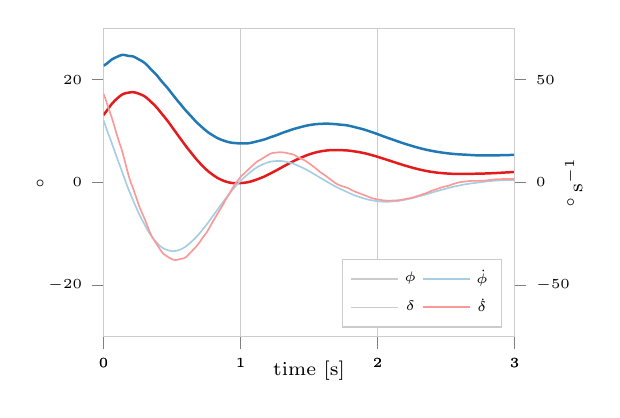
\begin{tikzpicture}

\definecolor{color2}{rgb}{0.650980412960052,0.807843148708344,0.890196084976196}
\definecolor{color1}{rgb}{0.890595931165359,0.104498271322718,0.111080354627441}
\definecolor{color3}{rgb}{0.983206460055183,0.598016170982052,0.594233010884594}
\definecolor{color0}{rgb}{0.125720876952012,0.473233373609244,0.707327968232772}

\begin{axis}[
xlabel={time [\si{\second}]},
ylabel={\si{\degree}},
xmin=0, xmax=3,
ymin=-30, ymax=30,
width=6.8cm,
height=5.5cm,
axis y line*=left,
tick align=outside,
xmajorgrids,
x grid style={white!80.0!black},
y grid style={white!80.0!black},
axis line style={white!80.0!black},
legend style={at={(0.97,0.03)}, anchor=south east, draw=white!80.0!black},
legend cell align={left},
%legend entries={{$\phi$},{$\delta$},{$\dot{\phi}$},{$\dot{\delta}$}}
]
\addplot [line width=0.9pt, color0]
table {%
0 22.6998023986816
0.01 22.8863353729248
0.02 23.0641956329346
0.03001 23.2497653961182
0.04001 23.4932327270508
0.05 23.7267360687256
0.06004 23.9241371154785
0.07 24.0823841094971
0.08 24.2190341949463
0.09 24.3394260406494
0.1 24.4548206329346
0.11 24.5710277557373
0.12 24.6938076019287
0.13 24.7842197418213
0.14 24.8190498352051
0.15005 24.8044605255127
0.16 24.7538642883301
0.17 24.6879253387451
0.18 24.6335144042969
0.19 24.6011333465576
0.2 24.5875549316406
0.21 24.5480785369873
0.22 24.4658374786377
0.23 24.3414630889893
0.24003 24.2016716003418
0.25001 24.046199798584
0.26 23.8973846435547
0.27 23.751049041748
0.28 23.6086349487305
0.29 23.4437637329102
0.30001 23.2458267211914
0.31001 23.0119209289551
0.32001 22.74485206604
0.33004 22.4634456634521
0.34 22.1801776885986
0.35 21.9013977050781
0.36 21.6357250213623
0.37 21.3734035491943
0.38 21.1023693084717
0.39 20.8070011138916
0.4 20.4777278900146
0.41001 20.1358680725098
0.42005 19.8058261871338
0.43 19.4895935058594
0.44 19.189826965332
0.45 18.8978214263916
0.46 18.5980663299561
0.47 18.278299331665
0.48 17.9417476654053
0.49 17.5955257415771
0.5 17.247444152832
0.51003 16.9105796813965
0.52 16.586145401001
0.53 16.2506141662598
0.54 15.9126825332642
0.55 15.596004486084
0.56 15.2823524475098
0.57 14.9574413299561
0.58001 14.6314878463745
0.59001 14.3090829849243
0.60004 13.99489402771
0.61 13.7018032073975
0.62 13.4225187301636
0.63 13.1402053833008
0.64 12.850754737854
0.65 12.5589160919189
0.66 12.2619676589966
0.67 11.9658651351929
0.68 11.689001083374
0.69002 11.4394359588623
0.7 11.1991367340088
0.71 10.9605703353882
0.72 10.7215814590454
0.73 10.4876098632812
0.74 10.2544631958008
0.75 10.0286169052124
0.76 9.81890201568604
0.77 9.63033866882324
0.78003 9.46014022827148
0.79 9.29472160339355
0.80001 9.1296272277832
0.81 8.96701908111572
0.82 8.80918121337891
0.83 8.66123867034912
0.84 8.53071594238281
0.85001 8.41482448577881
0.86001 8.31127834320068
0.87004 8.21340751647949
0.88 8.12223434448242
0.89 8.03340339660645
0.9 7.94898271560669
0.91 7.87358665466309
0.92 7.80935001373291
0.93 7.76011514663696
0.94 7.72160053253174
0.95 7.69182538986206
0.96 7.66712665557861
0.97 7.64456462860107
0.98 7.62677812576294
0.99 7.61746168136597
1 7.61224508285522
1.01 7.60383272171021
1.02 7.59379482269287
1.03 7.58790636062622
1.04 7.59235048294067
1.05 7.61136293411255
1.06 7.64322853088379
1.07 7.686607837677
1.08 7.73833656311035
1.09 7.7969536781311
1.1 7.86112594604492
1.11 7.92596101760864
1.12001 7.99372482299805
1.13001 8.06009197235107
1.14003 8.12519836425781
1.15 8.1914005279541
1.16 8.26171875
1.17 8.33746337890625
1.18 8.42459011077881
1.19 8.51809024810791
1.2 8.61777591705322
1.21 8.71939182281494
1.22 8.81791400909424
1.23002 8.90975475311279
1.24 8.99699211120605
1.25 9.08343982696533
1.26 9.17581939697266
1.27 9.27498245239258
1.28 9.37987899780273
1.29 9.48691463470459
1.3 9.59302234649658
1.31 9.69290637969971
1.32003 9.78672409057617
1.33 9.87504005432129
1.34 9.9652738571167
1.35001 10.0567855834961
1.36 10.1504125595093
1.37 10.2434930801392
1.38 10.3343315124512
1.39 10.4181604385376
1.40001 10.4945497512817
1.41004 10.5683288574219
1.42 10.6386728286743
1.43 10.7083082199097
1.44 10.7806510925293
1.45 10.8522882461548
1.46 10.9221601486206
1.47 10.9887571334839
1.48 11.050196647644
1.49 11.1037673950195
1.50004 11.1531467437744
1.51 11.1982946395874
1.52001 11.2401170730591
1.53 11.2778444290161
1.54 11.3108444213867
1.55 11.3396434783936
1.56 11.3641538619995
1.57 11.3841676712036
1.58001 11.3996477127075
1.59003 11.412971496582
1.6 11.4247961044312
1.61 11.4335041046143
1.62 11.4400520324707
1.63 11.440242767334
1.64 11.4356842041016
1.65 11.4236431121826
1.66001 11.4077215194702
1.67 11.3905944824219
1.68001 11.3742523193359
1.69 11.3566646575928
1.7 11.3319206237793
1.71 11.3001852035522
1.72 11.2690715789795
1.73 11.2424545288086
1.74 11.2205438613892
1.75 11.2004261016846
1.76 11.1752443313599
1.76999 11.1421270370483
1.78 11.0981531143188
1.79 11.0465173721313
1.80001 10.9875469207764
1.81 10.9235553741455
1.82 10.8577976226807
1.83 10.7916536331177
1.84 10.7268695831299
1.85 10.6624040603638
1.86003 10.5969543457031
1.87 10.5316972732544
1.88 10.462329864502
1.89 10.3891906738281
1.9 10.3105049133301
1.91 10.2269639968872
1.92 10.1389036178589
1.93 10.0489873886108
1.94 9.96004772186279
1.95003 9.87348365783691
1.96 9.78733348846436
1.97001 9.69868564605713
1.98 9.60665130615234
1.99 9.51150035858154
2 9.4137716293335
2.01 9.31384372711182
2.02 9.21220111846924
2.03 9.1103982925415
2.04004 9.01240730285645
2.05001 8.91515254974365
2.06 8.81983852386475
2.07 8.72530841827393
2.08 8.63300609588623
2.09 8.53981590270996
2.1 8.44566345214844
2.11 8.35137748718262
2.12 8.25704097747803
2.13003 8.16329383850098
2.14 8.07010841369629
2.15 7.97671270370483
2.16 7.88457345962524
2.17 7.79376602172852
2.18 7.703857421875
2.19 7.61555433273315
2.2 7.52949810028076
2.21 7.44688272476196
2.22003 7.36494779586792
2.23 7.28341436386108
2.24 7.20165491104126
2.25 7.12213611602783
2.26 7.04226684570312
2.27 6.96374607086182
2.28 6.88693428039551
2.29 6.81322050094604
2.3 6.74008655548096
2.31004 6.67019891738892
2.32 6.60125160217285
2.33001 6.53388690948486
2.34 6.46895217895508
2.35 6.40750741958618
2.36 6.34822416305542
2.37 6.29270839691162
2.38 6.23716497421265
2.39 6.18349075317383
2.4 6.13139533996582
2.41 6.08153057098389
2.42 6.03351449966431
2.43 5.98837614059448
2.44 5.94608163833618
2.45 5.90544271469116
2.46 5.86688089370728
2.47 5.82777214050293
2.48 5.78840637207031
2.49001 5.7519383430481
2.5 5.715576171875
2.51001 5.68225145339966
2.52 5.65194654464722
2.53 5.62373161315918
2.54 5.59748697280884
2.55 5.57279634475708
2.56 5.54883241653442
2.57 5.52618980407715
2.57999 5.50350427627563
2.59 5.48170137405396
2.6 5.46288299560547
2.61 5.45074224472046
2.62 5.44216394424438
2.63 5.42917203903198
2.64 5.41177129745483
2.65 5.39272737503052
2.66 5.37534141540527
2.67 5.36011838912964
2.68 5.34613084793091
2.69 5.33121061325073
2.7 5.31563472747803
2.71 5.30117511749268
2.72 5.2902364730835
2.73 5.28199672698975
2.74 5.27618598937988
2.75 5.27104330062866
2.76001 5.26795768737793
2.77 5.26662397384644
2.78001 5.26568222045898
2.79 5.26570844650269
2.8 5.26767158508301
2.81 5.26992750167847
2.82 5.27226543426514
2.83 5.27505970001221
2.84 5.27848672866821
2.84999 5.28174781799316
2.86 5.28429269790649
2.87 5.28737783432007
2.88 5.29120254516602
2.89001 5.29633092880249
2.9 5.30331516265869
2.91 5.31117153167725
2.92 5.31833934783936
2.93 5.32530164718628
2.94 5.33129835128784
2.95 5.33764839172363
2.96 5.34363317489624
2.97 5.35004043579102
2.98 5.35774660110474
2.99 5.36544275283813
3 5.37416791915894
3.01 5.38262176513672
3.02 5.39026594161987
3.03001 5.39761734008789
3.04001 5.40544128417969
3.05001 5.41306447982788
3.06001 5.42151403427124
3.07 5.4304723739624
3.08 5.43941783905029
3.09 5.44987964630127
3.1 5.45846652984619
3.11 5.46685552597046
3.11999 5.47587537765503
3.13 5.48394250869751
3.14 5.49179840087891
3.15 5.4986457824707
3.16001 5.50579404830933
3.17 5.51243591308594
3.18 5.5192232131958
3.19 5.52513837814331
3.2 5.53010892868042
3.21 5.53609657287598
3.22 5.54160833358765
3.23 5.54563617706299
3.24 5.5506649017334
3.25 5.55397510528564
3.26 5.55821084976196
3.27001 5.56030368804932
3.28 5.56331777572632
3.29 5.56638717651367
3.30001 5.56852674484253
3.31 5.57101583480835
3.32 5.57326698303223
3.33 5.57460927963257
3.34 5.57537841796875
3.35 5.57599258422852
3.36 5.57624435424805
3.37 5.57608127593994
3.38 5.57478904724121
3.38999 5.57427549362183
3.4 5.57445573806763
3.41 5.57287359237671
3.42 5.57154941558838
3.43 5.56965732574463
3.44 5.56624126434326
3.45 5.56178665161133
3.46 5.55584239959717
3.47 5.55298519134521
3.48 5.5481424331665
3.49 5.53938388824463
3.5 5.52447271347046
3.51 5.51191711425781
3.52 5.50326824188232
3.53 5.49857091903687
3.54 5.49203014373779
3.55 5.48189783096313
3.56 5.47390174865723
3.57001 5.46742391586304
3.58001 5.46107244491577
3.59 5.45246744155884
3.6 5.4449462890625
3.61 5.43724536895752
3.62 5.42737102508545
3.63 5.42003107070923
3.64 5.40911769866943
3.65 5.39945507049561
3.65999 5.38913345336914
3.67 5.3767671585083
3.68 5.36525106430054
3.69001 5.35189914703369
3.7 5.33846998214722
3.71 5.32434749603271
3.72 5.31053018569946
3.73 5.29591083526611
3.74 5.28008222579956
3.75 5.26373052597046
3.76 5.24699544906616
3.77 5.22870922088623
3.78 5.2093300819397
3.79 5.18924379348755
3.80001 5.16844606399536
3.81001 5.1489372253418
3.82001 5.13065814971924
3.83 5.11197471618652
3.84001 5.09437704086304
3.85001 5.07649183273315
3.86001 5.05830430984497
3.87001 5.03868770599365
3.88001 5.01788854598999
3.89001 4.99657678604126
3.90002 4.97506952285767
3.91 4.95422124862671
3.91999 4.93355417251587
3.92999 4.91394186019897
3.94 4.89242362976074
3.95 4.87017869949341
3.96 4.8472580909729
3.97 4.82316446304321
3.98 4.79831743240356
3.99 4.77250862121582
4 4.74725151062012
4.01 4.72189903259277
4.02 4.69701719284058
4.03 4.6716365814209
4.04 4.64657783508301
4.05 4.6204686164856
4.06 4.59545087814331
4.07 4.57016229629517
4.08 4.54461145401001
4.09 4.5184473991394
4.1 4.49340486526489
4.11001 4.4675612449646
4.12 4.44103384017944
4.13001 4.41372060775757
4.14 4.38739633560181
4.15 4.36092329025269
4.16 4.33490753173828
4.17 4.30911445617676
4.18 4.28386259078979
4.19 4.25803756713867
4.20001 4.23195171356201
4.21 4.20499277114868
4.22 4.17700719833374
4.23 4.1490626335144
4.24001 4.12109470367432
4.25 4.09336233139038
4.26 4.06473922729492
4.27 4.03607797622681
4.28 4.00836849212646
4.29002 3.98033428192139
4.30001 3.95221781730652
4.31 3.92424297332764
4.32 3.89602565765381
4.33 3.86810684204102
4.34001 3.84100008010864
4.35001 3.81428408622742
4.36001 3.78733348846436
4.37001 3.76050615310669
4.38003 3.73330664634705
4.39001 3.70822596549988
4.40001 3.68272924423218
4.41001 3.65744256973267
4.42001 3.63427925109863
4.43001 3.60936903953552
4.44001 3.58492422103882
4.45002 3.55953407287598
4.46001 3.53378534317017
4.47004 3.50881409645081
4.47999 3.48356509208679
4.49 3.45876836776733
4.5 3.43464851379395
4.51 3.4108772277832
4.52 3.38771367073059
4.53 3.36426734924316
4.54 3.34084796905518
4.55 3.31827807426453
4.56005 3.29666662216187
4.57 3.27491211891174
4.58 3.25383853912354
4.59 3.23440623283386
4.6 3.21359014511108
4.61 3.19375967979431
4.62 3.17477798461914
4.63 3.15432453155518
4.64 3.13579130172729
4.65006 3.11668872833252
4.66001 3.09789443016052
4.67 3.08043909072876
4.68001 3.06219935417175
4.69 3.04435777664185
4.7 3.02757358551025
4.71 3.01172852516174
4.72 2.99561858177185
4.73 2.9791738986969
4.74001 2.96269202232361
4.75 2.94765782356262
4.76 2.93056416511536
4.77 2.91398572921753
4.78001 2.89692521095276
4.79 2.88019990921021
4.8 2.8651876449585
4.81 2.8496527671814
4.82 2.83493280410767
4.83002 2.81866049766541
4.84 2.80428576469421
4.85 2.7885525226593
4.86 2.77336144447327
4.87 2.75811505317688
4.88 2.74329805374146
4.89001 2.72985911369324
4.90001 2.7163565158844
4.91001 2.7039909362793
4.92003 2.69186663627625
4.93001 2.68141341209412
4.94002 2.6708984375
4.95001 2.65957760810852
4.96001 2.64796495437622
4.97001 2.6370005607605
4.98001 2.62440204620361
4.99001 2.61223077774048
5 2.6013126373291
5.01004 2.58901810646057
5.01999 2.57760810852051
5.03 2.56688237190247
5.03999 2.55534768104553
5.05 2.54301309585571
5.06 2.53077936172485
5.07 2.51869797706604
5.08 2.5066339969635
5.09 2.49504613876343
5.10005 2.48362970352173
5.11 2.4718132019043
5.12 2.461590051651
5.13 2.45144271850586
5.14 2.44065046310425
5.15 2.43117475509644
5.16 2.42031407356262
5.17 2.41102766990662
5.18 2.40169477462769
5.19006 2.39248752593994
5.20001 2.38315963745117
5.21 2.37390518188477
5.22001 2.36463904380798
5.23 2.35628771781921
5.24 2.34457349777222
5.25 2.33295178413391
5.26 2.32042789459229
5.27 2.3102285861969
5.28001 2.29837393760681
5.29 2.28871154785156
5.3 2.27899646759033
5.31 2.26795434951782
5.32 2.25845575332642
5.33001 2.24649310112
5.34 2.23757076263428
5.35 2.2258882522583
5.36 2.21611547470093
5.37002 2.20512986183167
5.38 2.19221544265747
5.39 2.18122124671936
5.4 2.16943955421448
5.41 2.15642619132996
5.42 2.14402651786804
5.43001 2.13183856010437
5.44001 2.12088441848755
5.45001 2.11188077926636
5.46003 2.10270714759827
5.47001 2.09389042854309
5.48001 2.08636355400085
5.49001 2.07766652107239
5.50001 2.06829524040222
5.51001 2.0587272644043
5.52001 2.04734444618225
5.53001 2.03525924682617
5.54002 2.02347803115845
5.55004 2.01145482063293
5.55999 1.99844908714294
5.57 1.98687839508057
5.58 1.97523283958435
5.59 1.96255111694336
5.6 1.95099723339081
5.61001 1.94003927707672
5.62001 1.92763924598694
5.63001 1.91495800018311
5.64005 1.90282928943634
5.65 1.89212143421173
5.66 1.88145327568054
5.67001 1.87058091163635
5.68 1.85963475704193
5.69 1.84978127479553
5.7 1.83870661258698
5.71 1.82651555538177
5.72 1.81472170352936
5.73001 1.80418086051941
5.74 1.7929151058197
5.75 1.78090441226959
5.76 1.76947486400604
5.77 1.75823295116425
5.78001 1.74737417697906
5.79 1.73577129840851
5.8 1.72517085075378
5.81 1.71497428417206
5.82001 1.70383131504059
5.83001 1.69268989562988
5.84 1.68130266666412
5.85 1.66890239715576
5.86 1.6570497751236
5.87 1.64567255973816
5.88001 1.63469207286835
5.89001 1.62309634685516
5.9 1.61206185817719
5.91002 1.60232651233673
5.92 1.59304165840149
5.93001 1.58277773857117
5.94 1.57328307628632
5.95 1.56399893760681
5.96001 1.55322980880737
5.97 1.54220259189606
5.98 1.53118395805359
5.99 1.52001118659973
6.00003 1.5080943107605
6.01 1.49715542793274
6.02 1.48591208457947
6.03 1.47582840919495
6.04 1.46469807624817
6.05 1.45415699481964
6.06 1.44379138946533
6.07 1.43169045448303
6.08 1.42131078243256
6.09004 1.41023123264313
6.1 1.39895856380463
6.11 1.38850891590118
6.12 1.37774074077606
6.13 1.36660468578339
6.14 1.3548572063446
6.15 1.34406757354736
6.16001 1.33201241493225
6.17 1.32021534442902
6.18005 1.30962955951691
6.19 1.29796183109283
6.2 1.28616344928741
6.21 1.27386379241943
6.22 1.26182007789612
6.23001 1.2500216960907
6.24 1.23936378955841
6.25 1.22676813602448
6.26 1.21526408195496
6.27006 1.20328164100647
6.28 1.19091260433197
6.29 1.17976260185242
6.3 1.16841876506805
6.31 1.15667068958282
6.32 1.14357852935791
6.33 1.13117527961731
6.34 1.11849665641785
6.35 1.1062878370285
6.36 1.09251952171326
6.37 1.07883870601654
6.38 1.0660206079483
6.39 1.05290007591248
6.4 1.04069066047668
6.41 1.02721512317657
6.42 1.01440620422363
6.43001 1.00202167034149
6.44 0.989507794380188
6.45001 0.976535975933075
6.46 0.963996767997742
6.47001 0.952403724193573
6.48 0.940386354923248
6.49 0.928084492683411
6.5 0.915331900119781
6.51 0.902403771877289
6.52 0.888112545013428
6.53 0.875398278236389
6.53999 0.862548053264618
6.55 0.848468482494354
6.56 0.835597693920135
6.57 0.822896957397461
6.58 0.809500932693481
6.59 0.796542882919312
6.6 0.783372819423676
6.61 0.770220637321472
6.62 0.758346676826477
6.63 0.745202600955963
6.64 0.733220100402832
6.65 0.720459401607513
6.66 0.707778334617615
6.67 0.695420503616333
6.68 0.683535754680634
6.69 0.671425759792328
6.7 0.659491419792175
6.71 0.647679388523102
6.72001 0.636504292488098
6.73001 0.624830007553101
6.74001 0.612993538379669
6.75 0.601966321468353
6.76 0.591334998607635
6.77001 0.579904317855835
6.78 0.569167733192444
6.79 0.558499157428741
6.8 0.546895205974579
6.80999 0.535993337631226
6.82 0.524510502815247
6.83 0.51406455039978
6.84 0.503496944904327
6.85 0.492399394512177
6.86 0.482090026140213
6.87 0.471502751111984
6.88 0.462091267108917
6.89001 0.452008485794067
6.9 0.442253202199936
6.91 0.431253463029861
6.92 0.421417534351349
6.93 0.412397533655167
6.94 0.402156412601471
6.95 0.3926000893116
6.96 0.383056193590164
6.97 0.374688535928726
6.98 0.36629530787468
6.99001 0.357673972845078
7.00001 0.349311202764511
7.01001 0.341407805681229
7.02 0.33320751786232
7.03 0.325518101453781
7.04001 0.317994773387909
7.05 0.310037016868591
7.06 0.302411884069443
7.07 0.292319893836975
7.07999 0.282882362604141
7.09 0.274482548236847
7.1 0.265268743038177
7.11001 0.256359487771988
7.12 0.247896030545235
7.13 0.239900663495064
7.14 0.232589393854141
7.15 0.224256828427315
7.16001 0.216752037405968
7.17 0.208466365933418
7.18 0.202469497919083
7.19 0.195164054632187
7.2 0.18727020919323
7.21 0.179279744625092
7.22 0.172144338488579
7.23 0.163903579115868
7.24 0.154735133051872
7.25 0.148698702454567
7.26001 0.141196340322495
7.27001 0.134062334895134
7.28001 0.128933697938919
7.29001 0.123944126069546
7.3 0.119569905102253
7.31 0.115530595183372
7.32 0.110273435711861
7.33001 0.104240000247955
7.34 0.097172811627388
7.34999 0.0910946652293205
7.36 0.0829751268029213
7.37 0.0761226788163185
7.38 0.0705033391714096
7.39001 0.063368022441864
7.4 0.057514488697052
7.41 0.0508191809058189
7.42 0.0448561422526836
7.43 0.0370607934892178
7.44 0.0309291109442711
7.45 0.0258533321321011
7.46 0.0211227927356958
7.47 0.0149622028693557
7.48 0.00837327353656292
7.49 0.00315731950104237
7.5 -0.00302035245113075
7.51 -0.0103414747864008
7.52 -0.0157281700521708
7.53001 -0.0218055192381144
7.54 -0.0268026683479548
7.55 -0.0289844777435064
7.56 -0.03343715518713
7.57 -0.0376400128006935
7.58 -0.0430876985192299
7.59 -0.0478415712714195
7.6 -0.0537613295018673
7.61 -0.0606347098946571
7.61999 -0.0658965036273003
7.63 -0.0728507563471794
7.64 -0.080778032541275
7.65001 -0.0876153632998466
7.66 -0.0918365493416786
7.67 -0.0971459299325943
7.68 -0.102696642279625
7.69001 -0.10583584010601
7.7 -0.111336708068848
7.71 -0.115059554576874
7.72 -0.121600784361362
7.73 -0.128101468086243
7.74 -0.13400886952877
7.75 -0.140679359436035
7.76 -0.146805629134178
7.77 -0.153601244091988
7.78 -0.158811941742897
7.79 -0.16577385365963
7.80001 -0.16908498108387
7.81 -0.174252554774284
7.82001 -0.17862543463707
}; \label{plot_phi}
\addlegendentry{{$\phi$}}
]
\addplot [line width=0.9pt, color1]
table {%
0 13.1178455352783
0.01 13.4934568405151
0.02 13.8560762405396
0.03001 14.2125520706177
0.04001 14.5890789031982
0.05 14.9510278701782
0.06004 15.2832927703857
0.07 15.5847463607788
0.08 15.8632135391235
0.09 16.1206378936768
0.1 16.3625411987305
0.11 16.5928611755371
0.12 16.8159961700439
0.13 17.0119705200195
0.14 17.1675662994385
0.15005 17.2817783355713
0.16 17.3615226745605
0.17 17.4171009063721
0.18 17.4627838134766
0.19 17.5051765441895
0.2 17.5450000762939
0.21 17.5615768432617
0.22 17.5466938018799
0.23 17.4994354248047
0.24003 17.4310245513916
0.25001 17.3429183959961
0.26 17.2463722229004
0.27 17.1407909393311
0.28 17.0280742645264
0.29 16.8954010009766
0.30001 16.7374153137207
0.31001 16.5508403778076
0.32001 16.336030960083
0.33004 16.1003532409668
0.34 15.8531866073608
0.35 15.5988969802856
0.36 15.3431463241577
0.37 15.0819358825684
0.38 14.8102121353149
0.39 14.5198554992676
0.4 14.2051830291748
0.41001 13.8767824172974
0.42005 13.5458536148071
0.43 13.2152786254883
0.44 12.8878517150879
0.45 12.560736656189
0.46 12.2266206741333
0.47 11.8784799575806
0.48 11.5181884765625
0.49 11.1496305465698
0.5 10.7771158218384
0.51003 10.4066476821899
0.52 10.0409660339355
0.53 9.66841793060303
0.54 9.29453277587891
0.55 8.9322452545166
0.56 8.57191276550293
0.57 8.20553874969482
0.58001 7.83792209625244
0.59001 7.47156620025635
0.60004 7.10949897766113
0.61 6.76094102859497
0.62 6.42295265197754
0.63 6.08753490447998
0.64 5.75208950042725
0.65 5.41903352737427
0.66 5.08677005767822
0.67 4.75837135314941
0.68 4.44375228881836
0.69002 4.1465744972229
0.7 3.85840940475464
0.71 3.57645344734192
0.72 3.30000352859497
0.73 3.03173542022705
0.74 2.76808381080627
0.75 2.51240110397339
0.76 2.27003502845764
0.77 2.04465317726135
0.78003 1.83546054363251
0.79 1.63610804080963
0.80001 1.44418394565582
0.81 1.26010203361511
0.82 1.08488714694977
0.83 0.921128690242767
0.84 0.772716701030731
0.85001 0.637918412685394
0.86001 0.515176117420197
0.87004 0.401524424552917
0.88 0.298626780509949
0.89 0.204302817583084
0.9 0.119127668440342
0.91 0.0455421581864357
0.92 -0.0155856963247061
0.93 -0.0618082173168659
0.94 -0.0954855903983116
0.95 -0.11806134134531
0.96 -0.131628558039665
0.97 -0.138370409607887
0.98 -0.137280717492104
0.99 -0.126779347658157
1 -0.109361745417118
1.01 -0.0892366394400597
1.02 -0.0663330629467964
1.03 -0.0389534048736095
1.04 -0.00309295207262039
1.05 0.0437322482466698
1.06 0.100790567696095
1.07 0.167384192347527
1.08 0.24185873568058
1.09 0.323538929224014
1.1 0.41151362657547
1.11 0.503478407859802
1.12001 0.600641846656799
1.13001 0.699937343597412
1.14003 0.800307631492615
1.15 0.903079390525818
1.16 1.01053166389465
1.17 1.12348699569702
1.18 1.24529540538788
1.19 1.37338411808014
1.2 1.50759792327881
1.21 1.64552509784698
1.22 1.78451097011566
1.23002 1.92200398445129
1.24 2.05863642692566
1.25 2.19525003433228
1.26 2.33534455299377
1.27 2.48009467124939
1.28 2.62869238853455
1.29 2.77882552146912
1.3 2.92864155769348
1.31 3.07508373260498
1.32003 3.21817255020142
1.33 3.3585205078125
1.34 3.49943327903748
1.35001 3.64040040969849
1.36 3.78136873245239
1.37 3.92180037498474
1.38 4.06057500839233
1.39 4.19517803192139
1.40001 4.32445812225342
1.41004 4.44926357269287
1.42 4.56972694396973
1.43 4.68841791152954
1.44 4.80720138549805
1.45 4.92433547973633
1.46 5.03923273086548
1.47 5.15042972564697
1.48 5.25673913955688
1.49 5.35678577423096
1.50004 5.45167779922485
1.51 5.54189205169678
1.52001 5.62757253646851
1.53 5.70745849609375
1.54 5.7820463180542
1.55 5.85195350646973
1.56 5.91649293899536
1.57 5.97520303726196
1.58001 6.02773809432983
1.59003 6.07564735412598
1.6 6.12072086334229
1.61 6.16185426712036
1.62 6.19944334030151
1.63 6.2310938835144
1.64 6.2572193145752
1.65 6.27645635604858
1.66001 6.29070377349854
1.67 6.3011908531189
1.68001 6.30851030349731
1.69 6.31166362762451
1.7 6.30882501602173
1.71 6.30101776123047
1.72 6.29202651977539
1.73 6.28381443023682
1.74 6.2773380279541
1.75 6.2711501121521
1.76 6.26197719573975
1.76999 6.24775362014771
1.78 6.22726964950562
1.79 6.20187282562256
1.80001 6.17063665390015
1.81 6.13462924957275
1.82 6.09609889984131
1.83 6.05594301223755
1.84 6.0148344039917
1.85 5.97248458862305
1.86003 5.92754936218262
1.87 5.88175439834595
1.88 5.83247756958008
1.89 5.77980136871338
1.9 5.72265338897705
1.91 5.66165637969971
1.92 5.59653568267822
1.93 5.52849912643433
1.94 5.45914125442505
1.95003 5.38882446289062
1.96 5.31700992584229
1.97001 5.24237108230591
1.98 5.16479825973511
1.99 5.08477926254272
2 5.0027928352356
2.01 4.9189076423645
2.02 4.8332986831665
2.03 4.74666500091553
2.04004 4.66076755523682
2.05001 4.57462024688721
2.06 4.48904848098755
2.07 4.40328931808472
2.08 4.31777477264404
2.09 4.23199987411499
2.1 4.14578866958618
2.11 4.05953454971313
2.12 3.97319364547729
2.13003 3.88657736778259
2.14 3.80037498474121
2.15 3.71421813964844
2.16 3.62878131866455
2.17 3.54440879821777
2.18 3.46101832389832
2.19 3.37908625602722
2.2 3.29885244369507
2.21 3.22117209434509
2.22003 3.14441561698914
2.23 3.06818509101868
2.24 2.991854429245
2.25 2.91703915596008
2.26 2.84306693077087
2.27 2.77114725112915
2.28 2.70116424560547
2.29 2.6339328289032
2.3 2.56831812858582
2.31004 2.50542378425598
2.32 2.4443187713623
2.33001 2.38542246818542
2.34 2.32873296737671
2.35 2.27468872070312
2.36 2.2232358455658
2.37 2.17552971839905
2.38 2.12962174415588
2.39 2.08660840988159
2.4 2.04576206207275
2.41 2.00773119926453
2.42 1.97186732292175
2.43 1.93869352340698
2.44 1.90833652019501
2.45 1.88017058372498
2.46 1.85427665710449
2.47 1.82946705818176
2.48 1.80563056468964
2.49001 1.78408312797546
2.5 1.76324200630188
2.51001 1.74442136287689
2.52 1.72755491733551
2.53 1.71297204494476
2.54 1.70108413696289
2.55 1.69154918193817
2.56 1.68374931812286
2.57 1.67785406112671
2.57999 1.67317306995392
2.59 1.67047274112701
2.6 1.67030990123749
2.61 1.67389404773712
2.62 1.67950570583344
2.63 1.68262028694153
2.64 1.68380129337311
2.65 1.68441319465637
2.66 1.68623781204224
2.67 1.68923282623291
2.68 1.69314849376678
2.69 1.69637095928192
2.7 1.6990168094635
2.71 1.7018563747406
2.72 1.70611238479614
2.73 1.7113002538681
2.74 1.71751391887665
2.75 1.72383213043213
2.76001 1.73092865943909
2.77 1.73892092704773
2.78001 1.74685513973236
2.79 1.75496220588684
2.8 1.76411783695221
2.81 1.77406096458435
2.82 1.78479611873627
2.83 1.79663753509521
2.84 1.80921256542206
2.84999 1.82199013233185
2.86 1.83476936817169
2.87 1.84828650951385
2.88 1.86244428157806
2.89001 1.8771721124649
2.9 1.89241278171539
2.91 1.90849101543427
2.92 1.92451763153076
2.93 1.94070780277252
2.94 1.95581185817719
2.95 1.97069203853607
2.96 1.9855283498764
2.97 2.00103616714478
2.98 2.01751637458801
2.99 2.03409290313721
3 2.05122065544128
3.01 2.06787705421448
3.02 2.08418250083923
3.03001 2.10030841827393
3.04001 2.11677694320679
3.05001 2.13177919387817
3.06001 2.14576625823975
3.07 2.15962505340576
3.08 2.17395257949829
3.09 2.1896767616272
3.1 2.20479369163513
3.11 2.21977353096008
3.11999 2.23497319221497
3.13 2.24974822998047
3.14 2.26441097259521
3.15 2.27846503257751
3.16001 2.29239368438721
3.17 2.30479907989502
3.18 2.31695079803467
3.19 2.32887530326843
3.2 2.34033918380737
3.21 2.35233950614929
3.22 2.36408758163452
3.23 2.37500739097595
3.24 2.38664245605469
3.25 2.39757919311523
3.26 2.40879392623901
3.27001 2.41846919059753
3.28 2.4273509979248
3.29 2.4359827041626
3.30001 2.44324827194214
3.31 2.45049643516541
3.32 2.45757174491882
3.33 2.46402978897095
3.34 2.46979069709778
3.35 2.47518682479858
3.36 2.48009562492371
3.37 2.48434591293335
3.38 2.4872624874115
3.38999 2.49005699157715
3.4 2.49353337287903
3.41 2.49596786499023
3.42 2.49871945381165
3.43 2.50113296508789
3.44 2.50265955924988
3.45 2.50358843803406
3.46 2.50359606742859
3.47 2.50543689727783
3.48 2.50539398193359
3.49 2.50311994552612
3.5 2.49825429916382
3.51 2.49480557441711
3.52 2.49385738372803
3.53 2.49530577659607
3.54 2.49556612968445
3.55 2.49372267723083
3.56 2.49302792549133
3.57001 2.49268507957458
3.58001 2.49260783195496
3.59 2.49038410186768
3.6 2.48873233795166
3.61 2.48749256134033
3.62 2.48536729812622
3.63 2.48501873016357
3.64 2.48310852050781
3.65 2.48201203346252
3.65999 2.48058462142944
3.67 2.47864985466003
3.68 2.4775230884552
3.69001 2.47506904602051
3.7 2.47181916236877
3.71 2.4688503742218
3.72 2.46658849716187
3.73 2.46452975273132
3.74 2.46230268478394
3.75 2.46008992195129
3.76 2.45781898498535
3.77 2.4546103477478
3.78 2.45055770874023
3.79 2.44583415985107
3.80001 2.43917465209961
3.81001 2.43121385574341
3.82001 2.4222424030304
3.83 2.41181302070618
3.84001 2.40070700645447
3.85001 2.38875555992126
3.86001 2.37601375579834
3.87001 2.36191320419312
3.88001 2.34719848632812
3.89001 2.33180451393127
3.90002 2.31636571884155
3.91 2.30121159553528
3.91999 2.2867226600647
3.92999 2.27282547950745
3.94 2.25858545303345
3.95 2.24501872062683
3.96 2.23203039169312
3.97 2.21921682357788
3.98 2.20641756057739
3.99 2.19370794296265
4 2.18168187141418
4.01 2.16976809501648
4.02 2.15793681144714
4.03 2.14549517631531
4.04 2.13333868980408
4.05 2.120774269104
4.06 2.10907411575317
4.07 2.09739923477173
4.08 2.0854799747467
4.09 2.07328319549561
4.1 2.06156539916992
4.11001 2.04895186424255
4.12 2.0358464717865
4.13001 2.02217364311218
4.14 2.00776219367981
4.15 1.99318695068359
4.16 1.97886097431183
4.17 1.96456778049469
4.18 1.95068538188934
4.19 1.936847448349
4.20001 1.92323291301727
4.21 1.90937471389771
4.22 1.89511096477509
4.23 1.8808753490448
4.24001 1.8659747838974
4.25 1.8509738445282
4.26 1.8361804485321
4.27 1.82196307182312
4.28 1.80832421779633
4.29002 1.79448342323303
4.30001 1.780641913414
4.31 1.76632380485535
4.32 1.75171959400177
4.33 1.73701703548431
4.34001 1.72190701961517
4.35001 1.70522105693817
4.36001 1.68686389923096
4.37001 1.66734302043915
4.38003 1.64676177501678
4.39001 1.62662029266357
4.40001 1.60571730136871
4.41001 1.58452796936035
4.42001 1.56452298164368
4.43001 1.54359090328217
4.44001 1.52305543422699
4.45002 1.50196588039398
4.46001 1.4812536239624
4.47004 1.46156573295593
4.47999 1.44216358661652
4.49 1.4236398935318
4.5 1.40643441677094
4.51 1.3904801607132
4.52 1.3758978843689
4.53 1.36182403564453
4.54 1.34826564788818
4.55 1.33554911613464
4.56005 1.32363343238831
4.57 1.31198346614838
4.58 1.30039131641388
4.59 1.29029905796051
4.6 1.2800966501236
4.61 1.27082097530365
4.62 1.26217460632324
4.63 1.25315272808075
4.64 1.24547433853149
4.65006 1.23766505718231
4.66001 1.23042142391205
4.67 1.22371125221252
4.68001 1.21596097946167
4.69 1.20815396308899
4.7 1.20151817798615
4.71 1.19569790363312
4.72 1.18971240520477
4.73 1.18388617038727
4.74001 1.17822074890137
4.75 1.17367196083069
4.76 1.16845047473907
4.77 1.16401278972626
4.78001 1.15958905220032
4.79 1.15434324741364
4.8 1.15014040470123
4.81 1.14617490768433
4.82 1.14317154884338
4.83002 1.1397066116333
4.84 1.13744676113129
4.85 1.134605884552
4.86 1.13222241401672
4.87 1.12961506843567
4.88 1.12697184085846
4.89001 1.12418377399445
4.90001 1.11965823173523
4.91001 1.11422669887543
4.92003 1.10765969753265
4.93001 1.10114109516144
4.94002 1.09408986568451
4.95001 1.08644437789917
4.96001 1.07833778858185
4.97001 1.0705600976944
4.98001 1.0617299079895
4.99001 1.05347490310669
5 1.04612755775452
5.01004 1.03864097595215
5.01999 1.03209555149078
5.03 1.02674245834351
5.03999 1.02162909507751
5.05 1.01727426052094
5.06 1.01401400566101
5.07 1.01146578788757
5.08 1.00941479206085
5.09 1.00776445865631
5.10005 1.0060623884201
5.11 1.00423634052277
5.12 1.00260925292969
5.13 1.00100135803223
5.14 0.999184966087341
5.15 0.998298943042755
5.16 0.997050404548645
5.17 0.996919810771942
5.18 0.996967315673828
5.19006 0.99699741601944
5.20001 0.997034847736359
5.21 0.997020959854126
5.22001 0.996840059757233
5.23 0.995968163013458
5.24 0.993966519832611
5.25 0.992475926876068
5.26 0.99056750535965
5.27 0.989811480045319
5.28001 0.988053441047668
5.29 0.987255215644836
5.3 0.986449241638184
5.31 0.985118329524994
5.32 0.984986186027527
5.33001 0.983041286468506
5.34 0.982128202915192
5.35 0.980447828769684
5.36 0.980160534381866
5.37002 0.979692876338959
5.38 0.97838169336319
5.39 0.978010535240173
5.4 0.977268576622009
5.41 0.975754857063293
5.42 0.9744713306427
5.43001 0.972931742668152
5.44001 0.970238208770752
5.45001 0.966862797737122
5.46003 0.961908459663391
5.47001 0.9559685587883
5.48001 0.949719905853271
5.49001 0.9424067735672
5.50001 0.934344828128815
5.51001 0.925916433334351
5.52001 0.916459977626801
5.53001 0.906788527965546
5.54002 0.897311091423035
5.55004 0.888185501098633
5.55999 0.879516422748566
5.57 0.872555613517761
5.58 0.866297602653503
5.59 0.860077381134033
5.6 0.854827582836151
5.61001 0.850195705890656
5.62001 0.844448149204254
5.63001 0.838041067123413
5.64005 0.83160936832428
5.65 0.825890481472015
5.66 0.820061147212982
5.67001 0.813763320446014
5.68 0.807199656963348
5.69 0.801057457923889
5.7 0.794454038143158
5.71 0.787524461746216
5.72 0.781140387058258
5.73001 0.775257349014282
5.74 0.768835306167603
5.75 0.762722969055176
5.76 0.757161498069763
5.77 0.751567423343658
5.78001 0.745840311050415
5.79 0.739493250846863
5.8 0.733959078788757
5.81 0.729260265827179
5.82001 0.72467565536499
5.83001 0.720914721488953
5.84 0.717426359653473
5.85 0.713743686676025
5.86 0.710493326187134
5.87 0.70782595872879
5.88001 0.70536196231842
5.89001 0.70173579454422
5.9 0.697602033615112
5.91002 0.693751692771912
5.92 0.690440237522125
5.93001 0.687130451202393
5.94 0.684266269207001
5.95 0.681683778762817
5.96001 0.67835408449173
5.97 0.674817442893982
5.98 0.671610176563263
5.99 0.668798863887787
6.00003 0.665787577629089
6.01 0.662771284580231
6.02 0.659362256526947
6.03 0.656544804573059
6.04 0.653369605541229
6.05 0.65077418088913
6.06 0.648203670978546
6.07 0.644716501235962
6.08 0.642103850841522
6.09004 0.639100730419159
6.1 0.635803401470184
6.11 0.632786989212036
6.12 0.629629552364349
6.13 0.626383781433105
6.14 0.622876465320587
6.15 0.619721829891205
6.16001 0.615997314453125
6.17 0.611650884151459
6.18005 0.607442259788513
6.19 0.602843165397644
6.2 0.598439335823059
6.21 0.594006299972534
6.22 0.589628458023071
6.23001 0.584949851036072
6.24 0.580650389194489
6.25 0.57543021440506
6.26 0.570857107639313
6.27006 0.566007375717163
6.28 0.560804009437561
6.29 0.556139051914215
6.3 0.551249444484711
6.31 0.546219348907471
6.32 0.540673434734344
6.33 0.535999178886414
6.34 0.53090363740921
6.35 0.526168763637543
6.36 0.520528137683868
6.37 0.515069782733917
6.38 0.510041296482086
6.39 0.505160093307495
6.4 0.500569403171539
6.41 0.495075434446335
6.42 0.489758133888245
6.43001 0.484504610300064
6.44 0.478439331054688
6.45001 0.471503764390945
6.46 0.463889390230179
6.47001 0.456958562135696
6.48 0.449940741062164
6.49 0.442605197429657
6.5 0.434674888849258
6.51 0.426213949918747
6.52 0.417223304510117
6.53 0.409570872783661
6.53999 0.402143567800522
6.55 0.394323855638504
6.56 0.38657557964325
6.57 0.3790482878685
6.58 0.371569812297821
6.59 0.364704877138138
6.6 0.358129858970642
6.61 0.351617455482483
6.62 0.34556046128273
6.63 0.33905965089798
6.64 0.333305031061172
6.65 0.327248424291611
6.66 0.321107059717178
6.67 0.314699828624725
6.68 0.308682411909103
6.69 0.302460968494415
6.7 0.296435236930847
6.71 0.290757864713669
6.72001 0.284841686487198
6.73001 0.277837008237839
6.74001 0.270090281963348
6.75 0.26301521062851
6.76 0.256520211696625
6.77001 0.249623939394951
6.78 0.242365106940269
6.79 0.235394790768623
6.8 0.228410467505455
6.80999 0.222194418311119
6.82 0.216075763106346
6.83 0.211057931184769
6.84 0.205807402729988
6.85 0.199599102139473
6.86 0.194105640053749
6.87 0.188934534788132
6.88 0.184630587697029
6.89001 0.180234745144844
6.9 0.175732642412186
6.91 0.17101027071476
6.92 0.166741147637367
6.93 0.162891507148743
6.94 0.158283919095993
6.95 0.153717651963234
6.96 0.149129241704941
6.97 0.145252451300621
6.98 0.141331598162651
6.99001 0.137388229370117
7.00001 0.133061498403549
7.01001 0.127578929066658
7.02 0.121792703866959
7.03 0.116933390498161
7.04001 0.112213112413883
7.05 0.1077511459589
7.06 0.103678211569786
7.07 0.099001057446003
7.07999 0.0951551422476768
7.09 0.0919344574213028
7.1 0.0883904099464417
7.11001 0.085081122815609
7.12 0.0815069302916527
7.13 0.0781357809901237
7.14 0.0754947289824486
7.15 0.0725329294800758
7.16001 0.0700851455330849
7.17 0.0671847462654114
7.18 0.0656623467803001
7.19 0.0637024715542793
7.2 0.0615636184811592
7.21 0.0594198442995548
7.22 0.057795561850071
7.23 0.0556701458990574
7.24 0.0528285391628742
7.25 0.0516646727919579
7.26001 0.0495706535875797
7.27001 0.0470047034323215
7.28001 0.0443060174584389
7.29001 0.0406870916485786
7.3 0.0374290496110916
7.31 0.0350393727421761
7.32 0.0324388183653355
7.33001 0.0297896042466164
7.34 0.0264887418597937
7.34999 0.0235587544739246
7.36 0.0199328511953354
7.37 0.0171741899102926
7.38 0.0153342299163342
7.39001 0.0125069180503488
7.4 0.0102665098384023
7.41 0.00824632775038481
7.42 0.00707780616357923
7.43 0.00558478990569711
7.44 0.00479857344180346
7.45 0.00473688589408994
7.46 0.00461482396349311
7.47 0.00395887764170766
7.48 0.00283062737435102
7.49 0.0022108475677669
7.5 0.000833093537949026
7.51 -0.00136367056984454
7.52 -0.0026898430660367
7.53001 -0.00475357100367546
7.54 -0.00716356094926596
7.55 -0.00838023796677589
7.56 -0.0106670716777444
7.57 -0.0126965157687664
7.58 -0.0152352657169104
7.59 -0.0171263162046671
7.6 -0.0188617389649153
7.61 -0.0208950098603964
7.61999 -0.0218707881867886
7.63 -0.0235421042889357
7.64 -0.0256671812385321
7.65001 -0.0275197271257639
7.66 -0.029184315353632
7.67 -0.0313448756933212
7.68 -0.0333065092563629
7.69001 -0.0338697321712971
7.7 -0.035620428621769
7.71 -0.0359546840190887
7.72 -0.0376831851899624
7.73 -0.0392472632229328
7.74 -0.0402601584792137
7.75 -0.0415280684828758
7.76 -0.0426420047879219
7.77 -0.04425198584795
7.78 -0.0453299321234226
7.79 -0.0473290644586086
7.80001 -0.0483920387923717
7.81 -0.0510346069931984
7.82001 -0.0536478236317635
}; \label{plot_delta}
\addlegendentry{{$\delta$}}
\end{axis}

\begin{axis}[
ylabel={\si{\degree\per\second}},
xmin=0, xmax=3,
ymin=-75, ymax=75,
width=6.8cm,
height=5.5cm,
axis y line*=right,
tick align=outside,
%xmajorgrids,
x grid style={white!80.0!black},
y grid style={white!80.0!black},
axis line style={white!80.0!black},
legend style={at={(0.97,0.03)}, anchor=south east, draw=white!80.0!black},
legend transposed=true,
]
\addlegendimage{/pgfplots/refstyle=plot_phi}\addlegendentry{{$\phi$}}
\addlegendimage{/pgfplots/refstyle=plot_delta}\addlegendentry{{$\delta$}}
\addplot [semithick, color2]
table {%
0 30.1299896240234
0.01 28.2294578552246
0.02 26.3277454376221
0.03001 24.4552383422852
0.04001 22.6922149658203
0.05 20.9182243347168
0.06004 19.0935382843018
0.07 17.2222766876221
0.08 15.3416652679443
0.09 13.466007232666
0.1 11.6137733459473
0.11 9.79496002197266
0.12 8.0177583694458
0.13 6.21849822998047
0.14 4.36709117889404
0.15005 2.4876754283905
0.16 0.607674121856689
0.17 -1.23387014865875
0.18 -2.989422082901
0.19 -4.64382934570312
0.2 -6.21242380142212
0.21 -7.77824687957764
0.22 -9.35943603515625
0.23 -10.9481382369995
0.24003 -12.4929485321045
0.25001 -13.9943408966064
0.26 -15.4113912582397
0.27 -16.7580852508545
0.28 -18.0337619781494
0.29 -19.2849178314209
0.30001 -20.5240478515625
0.31001 -21.7492084503174
0.32001 -22.9502391815186
0.33004 -24.094274520874
0.34 -25.1638526916504
0.35 -26.1485271453857
0.36 -27.0364208221436
0.37 -27.8496074676514
0.38 -28.6092796325684
0.39 -29.3416213989258
0.4 -30.0577201843262
0.41001 -30.7191715240479
0.42005 -31.2831134796143
0.43 -31.7522220611572
0.44 -32.1269569396973
0.45 -32.4281578063965
0.46 -32.6820411682129
0.47 -32.9081535339355
0.48 -33.101619720459
0.49 -33.2514877319336
0.5 -33.3432388305664
0.51003 -33.3566780090332
0.52 -33.296070098877
0.53 -33.2044448852539
0.54 -33.0694961547852
0.55 -32.8503341674805
0.56 -32.5802536010742
0.57 -32.2835464477539
0.58001 -31.9430065155029
0.59001 -31.5541019439697
0.60004 -31.1161708831787
0.61 -30.610725402832
0.62 -30.0536689758301
0.63 -29.4778270721436
0.64 -28.8880367279053
0.65 -28.2799396514893
0.66 -27.6560935974121
0.67 -27.0095596313477
0.68 -26.3104610443115
0.69002 -25.5448837280273
0.7 -24.7534790039062
0.71 -23.9538478851318
0.72 -23.1488056182861
0.73 -22.3277816772461
0.74 -21.496410369873
0.75 -20.6483726501465
0.76 -19.773286819458
0.77 -18.8662433624268
0.78003 -17.9359188079834
0.79 -17.0100002288818
0.80001 -16.0928173065186
0.81 -15.1846237182617
0.82 -14.2793998718262
0.83 -13.3720636367798
0.84 -12.4494066238403
0.85001 -11.5172910690308
0.86001 -10.5836133956909
0.87004 -9.66385078430176
0.88 -8.76026439666748
0.89 -7.87787389755249
0.9 -7.01354312896729
0.91 -6.1615161895752
0.92 -5.3186616897583
0.93 -4.48190975189209
0.94 -3.65800595283508
0.95 -2.85135769844055
0.96 -2.07014417648315
0.97 -1.31486666202545
0.98 -0.584400594234467
0.99 0.12777279317379
1 0.814310014247894
1.01 1.4629157781601
1.02 2.08193039894104
1.03 2.68023633956909
1.04 3.26386284828186
1.05 3.84130835533142
1.06 4.40851926803589
1.07 4.9624490737915
1.08 5.49676418304443
1.09 6.00938940048218
1.1 6.49566411972046
1.11 6.94813823699951
1.12001 7.37070560455322
1.13001 7.76191425323486
1.14003 8.1200647354126
1.15 8.44913864135742
1.16 8.75211238861084
1.17 9.03234767913818
1.18 9.29929828643799
1.19 9.54521179199219
1.2 9.76844596862793
1.21 9.96296691894531
1.22 10.119345664978
1.23002 10.2362337112427
1.24 10.3160648345947
1.25 10.3739604949951
1.26 10.4143514633179
1.27 10.4398422241211
1.28 10.4500951766968
1.29 10.4411630630493
1.3 10.4073009490967
1.31 10.3400402069092
1.32003 10.2403240203857
1.33 10.1109523773193
1.34 9.96664142608643
1.35001 9.80931854248047
1.36 9.6373462677002
1.37 9.44611549377441
1.38 9.2357120513916
1.39 8.99796390533447
1.40001 8.73952293395996
1.41004 8.46853446960449
1.42 8.18166160583496
1.43 7.88177967071533
1.44 7.57840728759766
1.45 7.26535272598267
1.46 6.94176054000854
1.47 6.60867691040039
1.48 6.26179981231689
1.49 5.89785814285278
1.50004 5.52582979202271
1.51 5.14517402648926
1.52001 4.76186370849609
1.53 4.37437200546265
1.54 3.97997951507568
1.55 3.58040499687195
1.56 3.18215703964233
1.57 2.78194427490234
1.58001 2.38281106948853
1.59003 1.98265111446381
1.6 1.58625888824463
1.61 1.19171535968781
1.62 0.802170515060425
1.63 0.411429315805435
1.64 0.022874953225255
1.65 -0.367265909910202
1.66001 -0.751676023006439
1.67 -1.12633752822876
1.68001 -1.48406422138214
1.69 -1.83144974708557
1.7 -2.18222427368164
1.71 -2.5354380607605
1.72 -2.87437629699707
1.73 -3.19462943077087
1.74 -3.49818634986877
1.75 -3.78956198692322
1.76 -4.08139610290527
1.76999 -4.37824487686157
1.78 -4.68353271484375
1.79 -4.98998594284058
1.80001 -5.29072189331055
1.81 -5.58920001983643
1.82 -5.87657260894775
1.83 -6.15067434310913
1.84 -6.40800905227661
1.85 -6.65232944488525
1.86003 -6.88434839248657
1.87 -7.10439252853394
1.88 -7.31741571426392
1.89 -7.52318048477173
1.9 -7.72415018081665
1.91 -7.92004919052124
1.92 -8.10631370544434
1.93 -8.28142166137695
1.94 -8.43871879577637
1.95003 -8.5764627456665
1.96 -8.6987829208374
1.97001 -8.81036376953125
1.98 -8.91611862182617
1.99 -9.01405620574951
2 -9.10337829589844
2.01 -9.18280029296875
2.02 -9.25154399871826
2.03 -9.30669593811035
2.04004 -9.34169673919678
2.05001 -9.36361885070801
2.06 -9.3718090057373
2.07 -9.36487770080566
2.08 -9.34299755096436
2.09 -9.3148193359375
2.1 -9.27810478210449
2.11 -9.23252964019775
2.12 -9.17673683166504
2.13003 -9.11020755767822
2.14 -9.03559970855713
2.15 -8.95253562927246
2.16 -8.85941791534424
2.17 -8.75760173797607
2.18 -8.64840412139893
2.19 -8.53023052215576
2.2 -8.40258884429932
2.21 -8.26494026184082
2.22003 -8.12135791778564
2.23 -7.97013854980469
2.24 -7.81512546539307
2.25 -7.65206432342529
2.26 -7.49000024795532
2.27 -7.32330656051636
2.28 -7.15124559402466
2.29 -6.97323751449585
2.3 -6.79398775100708
2.31004 -6.60784149169922
2.32 -6.42204236984253
2.33001 -6.23299312591553
2.34 -6.04046058654785
2.35 -5.84183883666992
2.36 -5.64349889755249
2.37 -5.44271039962769
2.38 -5.24589776992798
2.39 -5.05070209503174
2.4 -4.85559749603271
2.41 -4.66100931167603
2.42 -4.46681451797485
2.43 -4.27291965484619
2.44 -4.0785608291626
2.45 -3.8873245716095
2.46 -3.69716787338257
2.47 -3.51443529129028
2.48 -3.33708262443542
2.49001 -3.15919041633606
2.5 -2.98522520065308
2.51001 -2.80989408493042
2.52 -2.63524293899536
2.53 -2.46621894836426
2.54 -2.30131149291992
2.55 -2.14114785194397
2.56 -1.9864205121994
2.57 -1.83727335929871
2.57999 -1.69581687450409
2.59 -1.56154799461365
2.6 -1.42682600021362
2.61 -1.28576123714447
2.62 -1.14470136165619
2.63 -1.0163459777832
2.64 -0.903548777103424
2.65 -0.798090994358063
2.66 -0.696230888366699
2.67 -0.595633685588837
2.68 -0.497764706611633
2.69 -0.405272483825684
2.7 -0.317899525165558
2.71 -0.231706827878952
2.72 -0.143240004777908
2.73 -0.0536040104925632
2.74 0.0362413823604584
2.75 0.122790180146694
2.76001 0.20963628590107
2.77 0.293658226728439
2.78001 0.377019613981247
2.79 0.456276595592499
2.8 0.535469114780426
2.81 0.606922090053558
2.82 0.673797070980072
2.83 0.735694229602814
2.84 0.794084131717682
2.84999 0.847677290439606
2.86 0.894232213497162
2.87 0.937802672386169
2.88 0.978687703609467
2.89001 1.01939737796783
2.9 1.05951726436615
2.91 1.09484589099884
2.92 1.12525272369385
2.93 1.15160799026489
2.94 1.17480158805847
2.95 1.19570434093475
2.96 1.20971012115479
2.97 1.22145938873291
2.98 1.23094093799591
2.99 1.2380450963974
3 1.24471020698547
3.01 1.24808192253113
3.02 1.24580514431
3.03001 1.24084258079529
3.04001 1.23420381546021
3.05001 1.23134124279022
3.06001 1.22937393188477
3.07 1.22184431552887
3.08 1.21126651763916
3.09 1.19953870773315
3.1 1.18315637111664
3.11 1.16499578952789
3.11999 1.14484477043152
3.13 1.12181556224823
3.14 1.09618604183197
3.15 1.06815350055695
3.16001 1.04021430015564
3.17 1.01380956172943
3.18 0.983805000782013
3.19 0.950076520442963
3.2 0.914214968681335
3.21 0.878428757190704
3.22 0.841095387935638
3.23 0.799962759017944
3.24 0.758706033229828
3.25 0.713656902313232
3.26 0.67071121931076
3.27001 0.62702339887619
3.28 0.584059596061707
3.29 0.542382955551147
3.30001 0.500214636325836
3.31 0.456883102655411
3.32 0.413650125265121
3.33 0.368953555822372
3.34 0.324403643608093
3.35 0.280979603528976
3.36 0.236834868788719
3.37 0.193561553955078
3.38 0.151802524924278
3.38999 0.109588012099266
3.4 0.0686743408441544
3.41 0.0253848936408758
3.42 -0.0173466522246599
3.43 -0.0599567368626595
3.44 -0.105110205709934
3.45 -0.15047325193882
3.46 -0.197756484150887
3.47 -0.240141123533249
3.48 -0.280624210834503
3.49 -0.3319271504879
3.5 -0.392313420772552
3.51 -0.447916567325592
3.52 -0.497462004423141
3.53 -0.538003087043762
3.54 -0.580423474311829
3.55 -0.628376960754395
3.56 -0.671990096569061
3.57001 -0.711134970188141
3.58001 -0.750744521617889
3.59 -0.788279116153717
3.6 -0.828314900398254
3.61 -0.868179440498352
3.62 -0.911202192306519
3.63 -0.950639724731445
3.64 -0.996039211750031
3.65 -1.03799867630005
3.65999 -1.08162295818329
3.67 -1.13062155246735
3.68 -1.17612612247467
3.69001 -1.22124493122101
3.7 -1.2673145532608
3.71 -1.3161655664444
3.72 -1.36520349979401
3.73 -1.41584885120392
3.74 -1.4691321849823
3.75 -1.52357709407806
3.76 -1.57776737213135
3.77 -1.63225877285004
3.78 -1.68818128108978
3.79 -1.7430145740509
3.80001 -1.79009068012238
3.81001 -1.83123409748077
3.82001 -1.86615240573883
3.83 -1.90030288696289
3.84001 -1.92660284042358
3.85001 -1.95299363136292
3.86001 -1.97621965408325
3.87001 -1.99991095066071
3.88001 -2.02413272857666
3.89001 -2.04539966583252
3.90002 -2.06612515449524
3.91 -2.08503341674805
3.91999 -2.10275721549988
3.92999 -2.11626648902893
3.94 -2.13492751121521
3.95 -2.15545535087585
3.96 -2.17782521247864
3.97 -2.20151615142822
3.98 -2.22515034675598
3.99 -2.25133085250854
4 -2.27601790428162
4.01 -2.29822564125061
4.02 -2.31979513168335
4.03 -2.33737754821777
4.04 -2.35761833190918
4.05 -2.37776756286621
4.06 -2.39676070213318
4.07 -2.41450309753418
4.08 -2.43131899833679
4.09 -2.44941568374634
4.1 -2.46347880363464
4.11001 -2.47681903839111
4.12 -2.4915988445282
4.13001 -2.50461173057556
4.14 -2.51224756240845
4.15 -2.52118706703186
4.16 -2.52773141860962
4.17 -2.53308463096619
4.18 -2.53720045089722
4.19 -2.54378724098206
4.20001 -2.54930210113525
4.21 -2.55625605583191
4.22 -2.56450200080872
4.23 -2.57094168663025
4.24001 -2.57234525680542
4.25 -2.57821726799011
4.26 -2.5849277973175
4.27 -2.59172010421753
4.28 -2.59485650062561
4.29002 -2.59844899177551
4.30001 -2.60073399543762
4.31 -2.60136890411377
4.32 -2.60205960273743
4.33 -2.60011959075928
4.34001 -2.59098100662231
4.35001 -2.57641506195068
4.36001 -2.55883836746216
4.37001 -2.53849768638611
4.38003 -2.51735877990723
4.39001 -2.48917698860168
4.40001 -2.45943212509155
4.41001 -2.42791819572449
4.42001 -2.39170169830322
4.43001 -2.35830521583557
4.44001 -2.32186460494995
4.45002 -2.28614687919617
4.46001 -2.25307655334473
4.47004 -2.21792483329773
4.47999 -2.18291926383972
4.49 -2.14811277389526
4.5 -2.11456894874573
4.51 -2.08217883110046
4.52 -2.04951024055481
4.53 -2.01755213737488
4.54 -1.98719644546509
4.55 -1.95527255535126
4.56005 -1.92240035533905
4.57 -1.89066576957703
4.58 -1.85622322559357
4.59 -1.82331001758575
4.6 -1.79444551467896
4.61 -1.76367330551147
4.62 -1.73285615444183
4.63 -1.70713222026825
4.64 -1.67865645885468
4.65006 -1.65230369567871
4.66001 -1.62566578388214
4.67 -1.59847092628479
4.68001 -1.56842231750488
4.69 -1.5428329706192
4.7 -1.51656460762024
4.71 -1.48991763591766
4.72 -1.46452951431274
4.73 -1.44114077091217
4.74001 -1.41969847679138
4.75 -1.39745426177979
4.76 -1.38141393661499
4.77 -1.36620032787323
4.78001 -1.35059928894043
4.79 -1.33356583118439
4.8 -1.31707894802094
4.81 -1.30375623703003
4.82 -1.29178655147552
4.83002 -1.28198313713074
4.84 -1.27166771888733
4.85 -1.26447224617004
4.86 -1.25798845291138
4.87 -1.25082159042358
4.88 -1.24337458610535
4.89001 -1.22954511642456
4.90001 -1.21281254291534
4.91001 -1.1921603679657
4.92003 -1.17045867443085
4.93001 -1.14485120773315
4.94002 -1.1196266412735
4.95001 -1.09621918201447
4.96001 -1.07230567932129
4.97001 -1.04711389541626
4.98001 -1.02514588832855
4.99001 -1.00356614589691
5 -0.981576442718506
5.01004 -0.961635053157806
5.01999 -0.943561196327209
5.03 -0.925183475017548
5.03999 -0.910805821418762
5.05 -0.901625514030457
5.06 -0.893573522567749
5.07 -0.886849582195282
5.08 -0.881074190139771
5.09 -0.875211656093597
5.10005 -0.868272960186005
5.11 -0.864330768585205
5.12 -0.854373812675476
5.13 -0.848678052425385
5.14 -0.844483613967896
5.15 -0.839521884918213
5.16 -0.838895797729492
5.17 -0.837130308151245
5.18 -0.835416197776794
5.19006 -0.834046900272369
5.20001 -0.833492279052734
5.21 -0.835089147090912
5.22001 -0.833987355232239
5.23 -0.831515073776245
5.24 -0.839199125766754
5.25 -0.847920656204224
5.26 -0.857214510440826
5.27 -0.862663686275482
5.28001 -0.870931208133698
5.29 -0.876259565353394
5.3 -0.881924986839294
5.31 -0.892604649066925
5.32 -0.90162318944931
5.33001 -0.909650027751923
5.34 -0.916485130786896
5.35 -0.930592060089111
5.36 -0.942456305027008
5.37002 -0.95657879114151
5.38 -0.975309729576111
5.39 -0.990295708179474
5.4 -1.00731372833252
5.41 -1.02634882926941
5.42 -1.04449415206909
5.43001 -1.05915772914886
5.44001 -1.06580424308777
5.45001 -1.06674921512604
5.46003 -1.06573343276978
5.47001 -1.06198608875275
5.48001 -1.05415892601013
5.49001 -1.04840910434723
5.50001 -1.04208087921143
5.51001 -1.03528034687042
5.52001 -1.03120172023773
5.53001 -1.02775740623474
5.54002 -1.02326011657715
5.55004 -1.02150988578796
5.55999 -1.02284693717957
5.57 -1.02222394943237
5.58 -1.0232093334198
5.59 -1.02611088752747
5.6 -1.02719354629517
5.61001 -1.02621114253998
5.62001 -1.02594470977783
5.63001 -1.02505564689636
5.64005 -1.02381789684296
5.65 -1.019158244133
5.66 -1.01441395282745
5.67001 -1.00781011581421
5.68 -1.00162708759308
5.69 -0.993815064430237
5.7 -0.988464117050171
5.71 -0.985635042190552
5.72 -0.982275903224945
5.73001 -0.974376559257507
5.74 -0.96924215555191
5.75 -0.967372417449951
5.76 -0.963471710681915
5.77 -0.958189427852631
5.78001 -0.949964284896851
5.79 -0.946077346801758
5.8 -0.94052129983902
5.81 -0.935793995857239
5.82001 -0.934740126132965
5.83001 -0.935284197330475
5.84 -0.936130583286285
5.85 -0.940307438373566
5.86 -0.943436324596405
5.87 -0.94648140668869
5.88001 -0.94781082868576
5.89001 -0.947302341461182
5.9 -0.945635437965393
5.91002 -0.941714584827423
5.92 -0.940171897411346
5.93001 -0.940391957759857
5.94 -0.939388155937195
5.95 -0.939405977725983
5.96001 -0.940567135810852
5.97 -0.943939387798309
5.98 -0.948582768440247
5.99 -0.954491198062897
6.00003 -0.961037218570709
6.01 -0.962789535522461
6.02 -0.968581140041351
6.03 -0.971072852611542
6.04 -0.9772047996521
6.05 -0.982329666614532
6.06 -0.987270474433899
6.07 -0.994848430156708
6.08 -1.00093626976013
6.09004 -1.00618469715118
6.1 -1.01247203350067
6.11 -1.01757800579071
6.12 -1.02356421947479
6.13 -1.03092479705811
6.14 -1.03895115852356
6.15 -1.04567384719849
6.16001 -1.05266785621643
6.17 -1.05801236629486
6.18005 -1.06086409091949
6.19 -1.06713771820068
6.2 -1.07520484924316
6.21 -1.08381128311157
6.22 -1.08984100818634
6.23001 -1.09425592422485
6.24 -1.09838044643402
6.25 -1.10547626018524
6.26 -1.11055111885071
6.27006 -1.11584603786469
6.28 -1.12053537368774
6.29 -1.12384247779846
6.3 -1.12754011154175
6.31 -1.13184058666229
6.32 -1.14025413990021
6.33 -1.1475750207901
6.34 -1.15211319923401
6.35 -1.15844869613647
6.36 -1.1665290594101
6.37 -1.17404818534851
6.38 -1.18158376216888
6.39 -1.18855321407318
6.4 -1.19322824478149
6.41 -1.19999384880066
6.42 -1.20516431331635
6.43001 -1.20745420455933
6.44 -1.20860123634338
6.45001 -1.20769250392914
6.46 -1.20543360710144
6.47001 -1.2035585641861
6.48 -1.20185661315918
6.49 -1.19844043254852
6.5 -1.19469487667084
6.51 -1.1897919178009
6.52 -1.19002401828766
6.53 -1.18677520751953
6.53999 -1.18381762504578
6.55 -1.18293607234955
6.56 -1.17586255073547
6.57 -1.17266142368317
6.58 -1.16929423809052
6.59 -1.16751289367676
6.6 -1.16502547264099
6.61 -1.16104996204376
6.62 -1.15584814548492
6.63 -1.15306067466736
6.64 -1.14818453788757
6.65 -1.14493560791016
6.66 -1.1401172876358
6.67 -1.13421452045441
6.68 -1.1287956237793
6.69 -1.12255549430847
6.7 -1.11732745170593
6.71 -1.11152505874634
6.72001 -1.10074877738953
6.73001 -1.08983492851257
6.74001 -1.07860350608826
6.75 -1.06813859939575
6.76 -1.05785930156708
6.77001 -1.0461038351059
6.78 -1.03198897838593
6.79 -1.02000641822815
6.8 -1.01082038879395
6.80999 -1.00088012218475
6.82 -0.992984652519226
6.83 -0.983438193798065
6.84 -0.972116410732269
6.85 -0.960855782032013
6.86 -0.951079845428467
6.87 -0.942337810993195
6.88 -0.931576430797577
6.89001 -0.922774374485016
6.9 -0.912934184074402
6.91 -0.906386256217957
6.92 -0.896758794784546
6.93 -0.887029945850372
6.94 -0.87828803062439
6.95 -0.867620468139648
6.96 -0.858134686946869
6.97 -0.846578180789948
6.98 -0.836333811283112
6.99001 -0.82549923658371
7.00001 -0.810147345066071
7.01001 -0.792425394058228
7.02 -0.778647124767303
7.03 -0.765734195709229
7.04001 -0.750629246234894
7.05 -0.739328622817993
7.06 -0.72703629732132
7.07 -0.723070442676544
7.07999 -0.7154860496521
7.09 -0.70786851644516
7.1 -0.701431274414062
7.11001 -0.693111062049866
7.12 -0.685216546058655
7.13 -0.676198780536652
7.14 -0.668888568878174
7.15 -0.663091540336609
7.16001 -0.654932796955109
7.17 -0.649850130081177
7.18 -0.640870809555054
7.19 -0.635848224163055
7.2 -0.631575882434845
7.21 -0.628967344760895
7.22 -0.624006390571594
7.23 -0.622495293617249
7.24 -0.6213618516922
7.25 -0.616187036037445
7.26001 -0.612020432949066
7.27001 -0.604724168777466
7.28001 -0.591244280338287
7.29001 -0.576828896999359
7.3 -0.565522313117981
7.31 -0.555259644985199
7.32 -0.546308100223541
7.33001 -0.539561450481415
7.34 -0.533746719360352
7.34999 -0.527178227901459
7.36 -0.524901449680328
7.37 -0.520981669425964
7.38 -0.516201078891754
7.39001 -0.511592209339142
7.4 -0.507264792919159
7.41 -0.505684018135071
7.42 -0.505273163318634
7.43 -0.508223593235016
7.44 -0.506839454174042
7.45 -0.50518798828125
7.46 -0.502599120140076
7.47 -0.504638969898224
7.48 -0.505019962787628
7.49 -0.504071056842804
7.5 -0.503262519836426
7.51 -0.506215810775757
7.52 -0.505036592483521
7.53001 -0.501824676990509
7.54 -0.496676325798035
7.55 -0.486883968114853
7.56 -0.482078373432159
7.57 -0.477041870355606
7.58 -0.475136458873749
7.59 -0.474010646343231
7.6 -0.475916534662247
7.61 -0.47917315363884
7.61999 -0.480243563652039
7.63 -0.484487354755402
7.64 -0.490431487560272
7.65001 -0.491445183753967
7.66 -0.487265706062317
7.67 -0.486716032028198
7.68 -0.487802237272263
7.69001 -0.483995258808136
7.7 -0.485611081123352
7.71 -0.485473722219467
7.72 -0.489512145519257
7.73 -0.495009630918503
7.74 -0.499872744083405
7.75 -0.505785405635834
7.76 -0.510482966899872
7.77 -0.515809714794159
7.78 -0.518039166927338
7.79 -0.52408492565155
7.80001 -0.517355620861053
7.81 -0.516736745834351
7.82001 -0.51256263256073
}; \addlegendentry{{$\dot{\phi}$}}
\addplot [semithick, color3]
table {%
0 43.007682800293
0.01 41.334774017334
0.02 39.3594932556152
0.03001 37.2314872741699
0.04001 35.3044471740723
0.05 33.4363899230957
0.06004 31.4889144897461
0.07 29.3712348937988
0.08 27.1402263641357
0.09 24.8022422790527
0.1 22.5627899169922
0.11 20.4463272094727
0.12 18.4730110168457
0.13 16.455904006958
0.14 14.2194576263428
0.15005 11.6932468414307
0.16 9.08409595489502
0.17 6.49325752258301
0.18 4.02407836914062
0.19 1.73662304878235
0.2 -0.21655210852623
0.21 -1.91759693622589
0.22 -3.72760534286499
0.23 -5.66428518295288
0.24003 -7.65292310714722
0.25001 -9.61797904968262
0.26 -11.5073251724243
0.27 -13.2094402313232
0.28 -14.7414712905884
0.29 -16.1848258972168
0.30001 -17.7246017456055
0.31001 -19.3905410766602
0.32001 -21.1872444152832
0.33004 -22.9240322113037
0.34 -24.4774723052979
0.35 -25.8859119415283
0.36 -27.1404628753662
0.37 -28.1930999755859
0.38 -29.1785316467285
0.39 -30.1492710113525
0.4 -31.219108581543
0.41001 -32.2978935241699
0.42005 -33.3319129943848
0.43 -34.1886863708496
0.44 -34.8439903259277
0.45 -35.3057327270508
0.46 -35.7377815246582
0.47 -36.1871490478516
0.48 -36.6167106628418
0.49 -36.9765739440918
0.5 -37.3129806518555
0.51003 -37.563232421875
0.52 -37.6514091491699
0.53 -37.6507835388184
0.54 -37.5351066589355
0.55 -37.3538360595703
0.56 -37.1816253662109
0.57 -37.0672912597656
0.58001 -36.9502029418945
0.59001 -36.7537727355957
0.60004 -36.345085144043
0.61 -35.7625427246094
0.62 -35.0853424072266
0.63 -34.3593940734863
0.64 -33.6867904663086
0.65 -32.9561958312988
0.66 -32.2843589782715
0.67 -31.5755043029785
0.68 -30.8052597045898
0.69002 -30.0503673553467
0.7 -29.1684875488281
0.71 -28.1624526977539
0.72 -27.1524333953857
0.73 -26.2120418548584
0.74 -25.3664798736572
0.75 -24.4708290100098
0.76 -23.4518661499023
0.77 -22.3311290740967
0.78003 -21.1387004852295
0.79 -19.8855571746826
0.80001 -18.7483005523682
0.81 -17.5794467926025
0.82 -16.4813232421875
0.83 -15.3557138442993
0.84 -14.255687713623
0.85001 -13.2112636566162
0.86001 -12.128381729126
0.87004 -10.9780550003052
0.88 -9.73943424224854
0.89 -8.56379222869873
0.9 -7.43248224258423
0.91 -6.30196857452393
0.92 -5.18215179443359
0.93 -4.02764177322388
0.94 -2.92187523841858
0.95 -1.8571709394455
0.96 -0.799909293651581
0.97 0.10084580630064
0.98 0.983062744140625
0.99 1.84867584705353
1 2.66967535018921
1.01 3.43815684318542
1.02 4.02404022216797
1.03 4.57897853851318
1.04 5.21824789047241
1.05 5.86515855789185
1.06 6.50971126556396
1.07 7.14678144454956
1.08 7.77784061431885
1.09 8.36313343048096
1.1 8.98576545715332
1.11 9.57995319366455
1.12001 10.151572227478
1.13001 10.5402040481567
1.14003 10.9062252044678
1.15 11.2744188308716
1.16 11.6917371749878
1.17 12.1120767593384
1.18 12.5536680221558
1.19 12.9519662857056
1.2 13.3527135848999
1.21 13.7095499038696
1.22 14.0480470657349
1.23002 14.2487440109253
1.24 14.4356651306152
1.25 14.4294137954712
1.26 14.5179347991943
1.27 14.6166067123413
1.28 14.6908712387085
1.29 14.6913890838623
1.3 14.6623296737671
1.31 14.6176462173462
1.32003 14.5581159591675
1.33 14.4564847946167
1.34 14.3362703323364
1.35001 14.1192617416382
1.36 13.9703378677368
1.37 13.8418092727661
1.38 13.6657409667969
1.39 13.4579610824585
1.40001 13.0663051605225
1.41004 12.6396636962891
1.42 12.2754383087158
1.43 11.9938640594482
1.44 11.6913270950317
1.45 11.3821897506714
1.46 11.0516052246094
1.47 10.6444063186646
1.48 10.2385578155518
1.49 9.81233882904053
1.50004 9.34319305419922
1.51 8.88641357421875
1.52001 8.34296798706055
1.53 7.81132555007935
1.54 7.32427597045898
1.55 6.86224794387817
1.56 6.26505470275879
1.57 5.69295644760132
1.58001 5.0940146446228
1.59003 4.65899610519409
1.6 4.22447681427002
1.61 3.78779554367065
1.62 3.32451272010803
1.63 2.82364344596863
1.64 2.32469177246094
1.65 1.81345820426941
1.66001 1.28733789920807
1.67 0.807424128055573
1.68001 0.248780518770218
1.69 -0.23024794459343
1.7 -0.594761192798615
1.71 -0.91045355796814
1.72 -1.25588762760162
1.73 -1.54399347305298
1.74 -1.76755607128143
1.75 -1.96971833705902
1.76 -2.16809129714966
1.76999 -2.37230944633484
1.78 -2.60714077949524
1.79 -2.88198733329773
1.80001 -3.32081866264343
1.81 -3.62806582450867
1.82 -3.93544864654541
1.83 -4.24171447753906
1.84 -4.54622030258179
1.85 -4.80680322647095
1.86003 -5.07166147232056
1.87 -5.29316425323486
1.88 -5.54425001144409
1.89 -5.79639482498169
1.9 -6.05579471588135
1.91 -6.295738697052
1.92 -6.61278581619263
1.93 -6.87220525741577
1.94 -7.13444757461548
1.95003 -7.38502168655396
1.96 -7.60572242736816
1.97001 -7.83066749572754
1.98 -7.9660496711731
1.99 -8.08540821075439
2 -8.19733715057373
2.01 -8.31458759307861
2.02 -8.43253898620605
2.03 -8.54886817932129
2.04004 -8.66097068786621
2.05001 -8.74051952362061
2.06 -8.75710010528564
2.07 -8.83502864837646
2.08 -8.86337375640869
2.09 -8.82726955413818
2.1 -8.80762767791748
2.11 -8.76999664306641
2.12 -8.75939083099365
2.13003 -8.75130462646484
2.14 -8.68471717834473
2.15 -8.63456439971924
2.16 -8.56913280487061
2.17 -8.47032642364502
2.18 -8.34161949157715
2.19 -8.2194299697876
2.2 -8.08646297454834
2.21 -7.92003202438354
2.22003 -7.77756118774414
2.23 -7.70577573776245
2.24 -7.59491014480591
2.25 -7.47035455703735
2.26 -7.23939275741577
2.27 -7.02720928192139
2.28 -6.83117866516113
2.29 -6.60693264007568
2.3 -6.37714672088623
2.31004 -6.18255043029785
2.32 -5.93183183670044
2.33001 -5.72901582717896
2.34 -5.51221656799316
2.35 -5.31189107894897
2.36 -5.04959678649902
2.37 -4.75959396362305
2.38 -4.47692775726318
2.39 -4.18228244781494
2.4 -3.93470549583435
2.41 -3.69876766204834
2.42 -3.48323631286621
2.43 -3.23677253723145
2.44 -3.01185894012451
2.45 -2.76914858818054
2.46 -2.55351161956787
2.47 -2.32829213142395
2.48 -2.13030385971069
2.49001 -1.96068370342255
2.5 -1.82523167133331
2.51001 -1.71164441108704
2.52 -1.551598072052
2.53 -1.29493522644043
2.54 -1.04560852050781
2.55 -0.808689415454865
2.56 -0.607066214084625
2.57 -0.394283294677734
2.57999 -0.198110014200211
2.59 0.0101357642561197
2.6 0.126521587371826
2.61 0.220672026276588
2.62 0.312340646982193
2.63 0.371245712041855
2.64 0.478436410427094
2.65 0.537753999233246
2.66 0.627994060516357
2.67 0.705066382884979
2.68 0.758620381355286
2.69 0.782228052616119
2.7 0.79484224319458
2.71 0.786173701286316
2.72 0.793493747711182
2.73 0.804612219333649
2.74 0.819552302360535
2.75 0.851998448371887
2.76001 0.859613656997681
2.77 0.924369752407074
2.78001 0.902893602848053
2.79 0.962125420570374
2.8 0.998050212860107
2.81 1.13132095336914
2.82 1.22993111610413
2.83 1.32141542434692
2.84 1.39856457710266
2.84999 1.45092225074768
2.86 1.53326165676117
2.87 1.5790923833847
2.88 1.60553216934204
2.89001 1.58628296852112
2.9 1.59808909893036
2.91 1.66638886928558
2.92 1.70333313941956
2.93 1.71618008613586
2.94 1.67603361606598
2.95 1.64722740650177
2.96 1.71112668514252
2.97 1.73412501811981
2.98 1.78250980377197
2.99 1.79060459136963
3 1.76297795772552
3.01 1.74699091911316
3.02 1.76740515232086
3.03001 1.74908828735352
3.04001 1.71409547328949
3.05001 1.53859686851501
3.06001 1.4040744304657
3.07 1.44823312759399
3.08 1.49019277095795
3.09 1.54838860034943
3.1 1.5465714931488
3.11 1.52260088920593
3.11999 1.52914202213287
3.13 1.50226926803589
3.14 1.48785614967346
3.15 1.43689024448395
3.16001 1.36335599422455
3.17 1.24080765247345
3.18 1.23074209690094
3.19 1.23750174045563
3.2 1.21660614013672
3.21 1.20380640029907
3.22 1.17719948291779
3.23 1.15945649147034
3.24 1.16270208358765
3.25 1.14310598373413
3.26 1.09273946285248
3.27001 0.93622612953186
3.28 0.884728789329529
3.29 0.796638906002045
3.30001 0.702485918998718
3.31 0.680272281169891
3.32 0.639572083950043
3.33 0.599373281002045
3.34 0.548329532146454
3.35 0.472626090049744
3.36 0.426997512578964
3.37 0.366247534751892
3.38 0.247687309980392
3.38999 0.234870657324791
3.4 0.21609565615654
3.41 0.195876285433769
3.42 0.177893042564392
3.43 0.141213566064835
3.44 0.126759260892868
3.45 0.0803192332386971
3.46 0.0450254343450069
3.47 0.0419858396053314
3.48 -0.0854610800743103
3.49 -0.0359685309231281
3.5 -0.0557876527309418
3.51 -0.0586887747049332
3.52 -0.0222995299845934
3.53 -0.0516288876533508
3.54 -0.0984599739313126
3.55 -0.137373119592667
3.56 -0.166687428951263
3.57001 -0.218206435441971
3.58001 -0.237658217549324
3.59 -0.378437697887421
3.6 -0.333864092826843
3.61 -0.314121812582016
3.62 -0.312024652957916
3.63 -0.284278929233551
3.64 -0.273348867893219
3.65 -0.294101566076279
3.65999 -0.293508559465408
3.67 -0.252050191164017
3.68 -0.285589158535004
3.69001 -0.401288658380508
3.7 -0.408665657043457
3.71 -0.3804030418396
3.72 -0.341996133327484
3.73 -0.322831213474274
3.74 -0.302363663911819
3.75 -0.293298244476318
3.76 -0.310009777545929
3.77 -0.385340481996536
3.78 -0.435924023389816
3.79 -0.520798087120056
3.80001 -0.778590977191925
3.81001 -0.980270683765411
3.82001 -1.15651416778564
3.83 -1.24155247211456
3.84001 -1.40089249610901
3.85001 -1.46208000183105
3.86001 -1.54165458679199
3.87001 -1.58173501491547
3.88001 -1.60317146778107
3.89001 -1.6547464132309
3.90002 -1.66757774353027
3.91 -1.62437725067139
3.91999 -1.58394396305084
3.92999 -1.57935845851898
3.94 -1.49979853630066
3.95 -1.41936862468719
3.96 -1.32971441745758
3.97 -1.2775616645813
3.98 -1.25911569595337
3.99 -1.21274900436401
4 -1.17272007465363
4.01 -1.2016853094101
4.02 -1.19216620922089
4.03 -1.29418683052063
4.04 -1.25583779811859
4.05 -1.26345157623291
4.06 -1.23043489456177
4.07 -1.24189651012421
4.08 -1.26689374446869
4.09 -1.26122558116913
4.1 -1.28973817825317
4.11001 -1.3469330072403
4.12 -1.35661375522614
4.13001 -1.43396842479706
4.14 -1.51059103012085
4.15 -1.50806725025177
4.16 -1.52427506446838
4.17 -1.52683961391449
4.18 -1.51397013664246
4.19 -1.44509553909302
4.20001 -1.44029140472412
4.21 -1.42614555358887
4.22 -1.41326940059662
4.23 -1.43261349201202
4.24001 -1.55294644832611
4.25 -1.45544838905334
4.26 -1.40221917629242
4.27 -1.3652104139328
4.28 -1.37811696529388
4.29002 -1.38482081890106
4.30001 -1.42440986633301
4.31 -1.45128321647644
4.32 -1.45745062828064
4.33 -1.4938051700592
4.34001 -1.64748239517212
4.35001 -1.81011927127838
4.36001 -1.94528102874756
4.37001 -2.03497195243835
4.38003 -2.07450246810913
4.39001 -2.12438583374023
4.40001 -2.16273093223572
4.41001 -2.16693329811096
4.42001 -2.15538835525513
4.43001 -2.10497164726257
4.44001 -2.09326791763306
4.45002 -2.06387233734131
4.46001 -1.95778965950012
4.47004 -1.88684237003326
4.47999 -1.82108592987061
4.49 -1.73350548744202
4.5 -1.60138547420502
4.51 -1.46498465538025
4.52 -1.36608827114105
4.53 -1.30370140075684
4.54 -1.21891498565674
4.55 -1.16793537139893
4.56005 -1.12719750404358
4.57 -1.09102165699005
4.58 -1.09641313552856
4.59 -1.00573527812958
4.6 -0.923582136631012
4.61 -0.894368290901184
4.62 -0.851776659488678
4.63 -0.776850998401642
4.64 -0.726915121078491
4.65006 -0.688810348510742
4.66001 -0.699772477149963
4.67 -0.664353787899017
4.68001 -0.764404714107513
4.69 -0.689895033836365
4.7 -0.643383085727692
4.71 -0.605818927288055
4.72 -0.571667075157166
4.73 -0.544285714626312
4.74001 -0.50413578748703
4.75 -0.461146831512451
4.76 -0.395270645618439
4.77 -0.339784324169159
4.78001 -0.382791489362717
4.79 -0.417956382036209
4.8 -0.366522759199142
4.81 -0.309762924909592
4.82 -0.227410569787025
4.83002 -0.239353343844414
4.84 -0.20343941450119
4.85 -0.192835688591003
4.86 -0.173818126320839
4.87 -0.205782026052475
4.88 -0.237231522798538
4.89001 -0.378073692321777
4.90001 -0.531402826309204
4.91001 -0.661869287490845
4.92003 -0.743060767650604
4.93001 -0.80284982919693
4.94002 -0.822577178478241
4.95001 -0.818283379077911
4.96001 -0.827705144882202
4.97001 -0.837681114673615
4.98001 -0.81904262304306
4.99001 -0.780220091342926
5 -0.692450821399689
5.01004 -0.670363187789917
5.01999 -0.563872754573822
5.03 -0.491908252239227
5.03999 -0.393294632434845
5.05 -0.263480186462402
5.06 -0.182826697826385
5.07 -0.117259971797466
5.08 -0.0821167156100273
5.09 -0.062152873724699
5.10005 -0.0962077155709267
5.11 -0.0854687094688416
5.12 -0.170911401510239
5.13 -0.128291130065918
5.14 -0.10918977111578
5.15 -0.0808649286627769
5.16 -0.0415848195552826
5.17 0.00550856115296483
5.18 0.00385791552253067
5.19006 -0.0113864680752158
5.20001 -0.0421663299202919
5.21 -0.017360333353281
5.22001 -0.105698257684708
5.23 -0.127582877874374
5.24 -0.0714342296123505
5.25 -0.0228358004242182
5.26 -0.035000029951334
5.27 -0.0485212244093418
5.28001 -0.0858460366725922
5.29 -0.0912922546267509
5.3 -0.111414447426796
5.31 -0.0686808377504349
5.32 -0.0343042351305485
5.33001 -0.17209529876709
5.34 -0.133109241724014
5.35 -0.0776071771979332
5.36 -0.0239507034420967
5.37002 -0.0266071613878012
5.38 -0.0178281720727682
5.39 -0.0309532172977924
5.4 -0.044703796505928
5.41 -0.0688760951161385
5.42 -0.0933796539902687
5.43001 -0.209921285510063
5.44001 -0.409878522157669
5.45001 -0.565074443817139
5.46003 -0.693367660045624
5.47001 -0.797821521759033
5.48001 -0.874058485031128
5.49001 -0.89802759885788
5.50001 -0.93064934015274
5.51001 -0.943635880947113
5.52001 -0.939366281032562
5.53001 -0.933416843414307
5.54002 -0.914124131202698
5.55004 -0.823107600212097
5.55999 -0.727349102497101
5.57 -0.657261312007904
5.58 -0.575051486492157
5.59 -0.522227227687836
5.6 -0.482530564069748
5.61001 -0.49789896607399
5.62001 -0.551016449928284
5.63001 -0.598917543888092
5.64005 -0.597559750080109
5.65 -0.615956485271454
5.66 -0.618518710136414
5.67001 -0.666634738445282
5.68 -0.678335607051849
5.69 -0.658224761486053
5.7 -0.632367014884949
5.71 -0.596785306930542
5.72 -0.568259537220001
5.73001 -0.607104778289795
5.74 -0.57622629404068
5.75 -0.521424174308777
5.76 -0.513709843158722
5.77 -0.53226512670517
5.78001 -0.602058708667755
5.79 -0.545809745788574
5.8 -0.499732196331024
5.81 -0.443159401416779
5.82001 -0.369124919176102
5.83001 -0.303556174039841
5.84 -0.279740214347839
5.85 -0.237484723329544
5.86 -0.217218011617661
5.87 -0.205552011728287
5.88001 -0.242901429533958
5.89001 -0.335398733615875
5.9 -0.383282333612442
5.91002 -0.408269852399826
5.92 -0.348615497350693
5.93001 -0.334744065999985
5.94 -0.326820641756058
5.95 -0.29286327958107
5.96001 -0.324934154748917
5.97 -0.29641380906105
5.98 -0.252879440784454
5.99 -0.217019438743591
6.00003 -0.233820036053658
6.01 -0.328547805547714
6.02 -0.292145609855652
6.03 -0.30263289809227
6.04 -0.273263514041901
6.05 -0.269092559814453
6.06 -0.264600187540054
6.07 -0.284319013357162
6.08 -0.252414613962173
6.09004 -0.304155111312866
6.1 -0.323208808898926
6.11 -0.326123148202896
6.12 -0.326023191213608
6.13 -0.313012838363647
6.14 -0.323276817798615
6.15 -0.311284095048904
6.16001 -0.379673063755035
6.17 -0.436756998300552
6.18005 -0.4696044921875
6.19 -0.462032377719879
6.2 -0.414400160312653
6.21 -0.393799990415573
6.22 -0.439439177513123
6.23001 -0.493694305419922
6.24 -0.46808049082756
6.25 -0.463127434253693
6.26 -0.459012150764465
6.27006 -0.476451009511948
6.28 -0.523095786571503
6.29 -0.529076874256134
6.3 -0.521349966526031
6.31 -0.517584562301636
6.32 -0.462362557649612
6.33 -0.432004600763321
6.34 -0.494356870651245
6.35 -0.468794375658035
6.36 -0.472402989864349
6.37 -0.493228256702423
6.38 -0.45245623588562
6.39 -0.470315456390381
6.4 -0.495313256978989
6.41 -0.50701767206192
6.42 -0.514505684375763
6.43001 -0.579263389110565
6.44 -0.633129239082336
6.45001 -0.735296845436096
6.46 -0.777818262577057
6.47001 -0.743509709835052
6.48 -0.725529432296753
6.49 -0.758671343326569
6.5 -0.789923667907715
6.51 -0.822458863258362
6.52 -0.753091156482697
6.53 -0.722614109516144
6.53999 -0.700422585010529
6.55 -0.68743109703064
6.56 -0.760760247707367
6.57 -0.684327781200409
6.58 -0.674231588840485
6.59 -0.599321067333221
6.6 -0.583533346652985
6.61 -0.617713809013367
6.62 -0.594745576381683
6.63 -0.581180214881897
6.64 -0.574164271354675
6.65 -0.565575897693634
6.66 -0.596224725246429
6.67 -0.609208464622498
6.68 -0.581645905971527
6.69 -0.588609993457794
6.7 -0.554679691791534
6.71 -0.551533758640289
6.72001 -0.642373204231262
6.73001 -0.706971943378448
6.74001 -0.736321747303009
6.75 -0.695305287837982
6.76 -0.642715394496918
6.77001 -0.688401460647583
6.78 -0.712944030761719
6.79 -0.668755352497101
6.8 -0.612742245197296
6.80999 -0.564137637615204
6.82 -0.507552206516266
6.83 -0.485459268093109
6.84 -0.52549946308136
6.85 -0.549074113368988
6.86 -0.491884976625443
6.87 -0.451997637748718
6.88 -0.432667374610901
6.89001 -0.414422005414963
6.9 -0.400403618812561
6.91 -0.387327790260315
6.92 -0.403631329536438
6.93 -0.38047868013382
6.94 -0.399333298206329
6.95 -0.426130533218384
6.96 -0.414802134037018
6.97 -0.414167195558548
6.98 -0.37527146935463
6.99001 -0.387259185314178
7.00001 -0.512253224849701
7.01001 -0.593901813030243
7.02 -0.542795121669769
7.03 -0.474258184432983
7.04001 -0.477550506591797
7.05 -0.413095951080322
7.06 -0.382029682397842
7.07 -0.269641369581223
7.07999 -0.283063173294067
7.09 -0.24696347117424
7.1 -0.239271804690361
7.11001 -0.293299049139023
7.12 -0.278781205415726
7.13 -0.279685795307159
7.14 -0.214475125074387
7.15 -0.187135130167007
7.16001 -0.208064377307892
7.17 -0.18109342455864
7.18 -0.170921698212624
7.19 -0.139350548386574
7.2 -0.142899826169014
7.21 -0.111629121005535
7.22 -0.12890413403511
7.23 -0.114806942641735
7.24 -0.140667140483856
7.25 -0.123818069696426
7.26001 -0.167672201991081
7.27001 -0.261252582073212
7.28001 -0.368640899658203
7.29001 -0.431622952222824
7.3 -0.352213382720947
7.31 -0.268997728824615
7.32 -0.252809882164001
7.33001 -0.240423515439034
7.34 -0.25776132941246
7.34999 -0.232123285531998
7.36 -0.214397266507149
7.37 -0.192428022623062
7.38 -0.149636268615723
7.39001 -0.190800458192825
7.4 -0.141485914587975
7.41 -0.104449033737183
7.42 -0.0229727197438478
7.43 0.00108841201290488
7.44 -0.0225741062313318
7.45 -0.0181467365473509
7.46 -0.0257486049085855
7.47 0.00572983035817742
7.48 -0.0439645200967789
7.49 -0.0496757887303829
7.5 -0.106794625520706
7.51 -0.0954577475786209
7.52 -0.101141631603241
7.53001 -0.202943325042725
7.54 -0.243217170238495
7.55 -0.25079482793808
7.56 -0.241625040769577
7.57 -0.234621986746788
7.58 -0.209547966718674
7.59 -0.135073482990265
7.6 -0.0886199474334717
7.61 -0.0746650844812393
7.61999 -0.0568080097436905
7.63 -0.0551651455461979
7.64 -0.0648973807692528
7.65001 -0.163181141018867
7.66 -0.196273788809776
7.67 -0.179266482591629
7.68 -0.146798133850098
7.69001 -0.148470431566238
7.7 -0.120953008532524
7.71 -0.0832693353295326
7.72 -0.0918537154793739
7.73 -0.0625726655125618
7.74 -0.0393613018095493
7.75 -0.0472566373646259
7.76 -0.0585012100636959
7.77 -0.0874370709061623
7.78 -0.106674015522003
7.79 -0.107118591666222
7.80001 -0.257536172866821
7.81 -0.270008325576782
7.82001 -0.325654089450836
}; \addlegendentry{{$\dot{\delta}$}}
\end{axis}

\end{tikzpicture}

    \caption{Bicycle simulator}
    \label{fig:state_ph}
\end{subfigure}
\hfill
\begin{subfigure}{0.45\textwidth}
    \centering
    \captionsetup{width=\linewidth}
    % This file was created by matplotlib2tikz v0.6.2.
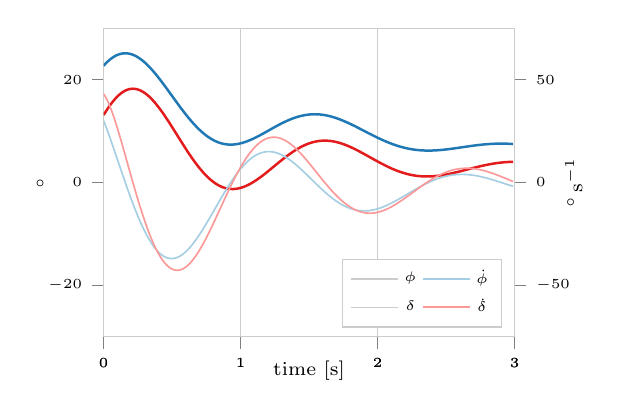
\begin{tikzpicture}

\definecolor{color2}{rgb}{0.650980412960052,0.807843148708344,0.890196084976196}
\definecolor{color1}{rgb}{0.890595931165359,0.104498271322718,0.111080354627441}
\definecolor{color3}{rgb}{0.983206460055183,0.598016170982052,0.594233010884594}
\definecolor{color0}{rgb}{0.125720876952012,0.473233373609244,0.707327968232772}

\begin{axis}[
xlabel={time [\si{\second}]},
ylabel={\si{\degree}},
xmin=0, xmax=3,
ymin=-30, ymax=30,
width=6.8cm,
height=5.5cm,
axis y line*=left,
tick align=outside,
xmajorgrids,
x grid style={white!80.0!black},
y grid style={white!80.0!black},
axis line style={white!80.0!black},
legend style={at={(0.97,0.03)}, anchor=south east, draw=white!80.0!black},
legend cell align={left},
%legend entries={{$\phi$},{$\delta$},{$\dot{\phi}$},{$\dot{\delta}$}}
]
\addplot [line width=0.9pt, color0]
table {%
0 22.6998024423626
0.0100000004749745 22.9924605507726
0.020000000949949 23.2675455985082
0.0300000014249235 23.524655984012
0.0400000018998981 23.7634336163698
0.0500000023748726 23.9835639272118
0.0600000028498471 24.1847757999382
0.0700000033248216 24.3668414168747
0.0800000037997961 24.5295760252264
0.0900000042747706 24.6728376229452
0.100000004749745 24.7965265658507
0.11000000522472 24.900585097554
0.120000005699694 24.9849968039308
0.130000006174669 25.0497859940647
0.140000006649643 25.0950170097534
0.150000007124618 25.1207934658189
0.160000007599592 25.127257423606
0.170000008074567 25.1145885001835
0.180000008549541 25.0830029158792
0.190000009024516 25.0327524828876
0.20000000949949 24.9641235377898
0.210000009974465 24.8774358209081
0.220000010449439 24.7730413054993
0.230000010924414 24.6513229798597
0.240000011399388 24.5126935854717
0.250000011874363 24.3575943143765
0.260000012349337 24.1864934689977
0.270000012824312 23.9998850876758
0.280000013299286 23.7982875391988
0.290000013774261 23.5822420896341
0.300000014249235 23.3523114447741
0.31000001472421 23.1090782715152
0.320000015199184 22.8531437014804
0.330000015674159 22.5851258201885
0.340000016149133 22.3056581450512
0.350000016624108 22.0153880954564
0.360000017099082 21.7149754581611
0.370000017574057 21.4050908511829
0.380000018049031 21.0864141893309
0.390000018524006 20.7596331544693
0.400000018998981 20.4254416735487
0.410000019473955 20.0845384073816
0.42000001994893 19.7376252530671
0.430000020423904 19.3854058629036
0.440000020898879 19.0285841825474
0.450000021373853 18.6678630110959
0.460000021848828 18.3039425856884
0.470000022323802 17.937519193129
0.480000022798777 17.5692838109399
0.490000023273751 17.1999207801613
0.500000023748726 16.8301065121096
0.5100000242237 16.4605082312058
0.520000024698675 16.0917827558782
0.530000025173649 15.7245753194371
0.540000025648624 15.3595184327066
0.550000026123598 14.997230790088
0.560000026598573 14.6383162206145
0.570000027073547 14.2833626854413
0.580000027548522 13.9329413230981
0.590000028023496 13.5876055437144
0.600000028498471 13.2478901733084
0.610000028973445 12.9143106491127
0.62000002944842 12.5873622667903
0.630000029923394 12.2675194802761
0.640000030398369 11.9552352548599
0.650000030873343 11.6509404740103
0.660000031348318 11.35504340032
0.670000031823292 11.0679291908389
0.680000032298267 10.7899594669436
0.690000032773241 10.5214719387832
0.700000033248216 10.2627800842237
0.71000003372319 10.0141728821081
0.720000034198165 9.77591459954012
0.730000034673139 9.54824463279197
0.740000035148114 9.33137740133664
0.750000035623088 9.12550229440239
0.760000036098063 8.93078366935021
0.770000036573038 8.74736090108018
0.780000037048012 8.57534848158067
0.790000037522987 8.41483616864621
0.800000037997961 8.26588918270409
0.810000038472936 8.1285484506087
0.82000003894791 8.00283089518396
0.830000039422885 7.88872976921994
0.840000039897859 7.78621503255932
0.850000040372834 7.69523377084215
0.860000040847808 7.61571065441473
0.870000041322783 7.54754843584978
0.880000041797757 7.49062848446984
0.890000042272732 7.44481135621561
0.900000042747706 7.40993739715422
0.910000043222681 7.38582737888029
0.920000043697655 7.37228316402424
0.93000004417263 7.36908840004886
0.940000044647604 7.3760092394851
0.950000045122579 7.39279508473299
0.960000045597553 7.41917935553206
0.970000046072528 7.45488027718878
0.980000046547502 7.49960168763581
0.990000047022477 7.55303386138871
1.00000004749745 7.61485434846156
1.01000004797243 7.68472882630191
1.0200000484474 7.7623119628091
1.03000004892237 7.84724828850688
1.04000004939735 7.93917307595269
1.05000004987232 8.03771322448034
1.0600000503473 8.14248814839142
1.07000005082227 8.25311066673285
1.08000005129725 8.36918789282315
1.09000005177222 8.49032212171912
1.1000000522472 8.61611171384619
1.11000005272217 8.74615197305143
1.12000005319715 8.88003601737587
1.13000005367212 9.01735564088402
1.14000005414709 9.15770216493236
1.15000005462207 9.30066727730482
1.16000005509704 9.4458438576923
1.17000005557202 9.59282678804441
1.18000005604699 9.7412137463753
1.19000005652197 9.89060598266071
1.20000005699694 10.040609075521
1.21000005747192 10.1908336684443
1.22000005794689 10.340896184364
1.23000005842187 10.4904195174688
1.24000005889684 10.6390337011846
1.25000005937181 10.7863765513358
1.26000005984679 10.9320942835557
1.27000006032176 11.0758421040856
1.28000006079674 11.2172847731673
1.29000006127171 11.3560971403042
1.30000006174669 11.4919646507316
1.31000006222166 11.624583822509
1.32000006269664 11.7536626937129
1.33000006317161 11.8789212392801
1.34000006364658 12.0000917571191
1.35000006412156 12.1169192231745
1.36000006459653 12.229161615201
1.37000006507151 12.3365902050667
1.38000006554648 12.4389898194752
1.39000006602146 12.5361590690619
1.40000006649643 12.6279105458827
1.41000006697141 12.7140709893811
1.42000006744638 12.794481420979
1.43000006792136 12.8689972475002
1.44000006839633 12.9374883336958
1.4500000688713 12.9998390441993
1.46000006934628 13.055948255295
1.47000006982125 13.1057293369423
1.48000007029623 13.1491101055477
1.4900000707712 13.1860327480337
1.50000007124618 13.2164537177981
1.51000007172115 13.2403436032102
1.52000007219613 13.2576869693337
1.5300000726711 13.2684821736105
1.54000007314608 13.2727411562822
1.55000007362105 13.2704892063643
1.56000007409602 13.2617647040266
1.570000074571 13.2466188402679
1.58000007504597 13.2251153148047
1.59000007552095 13.197330013125
1.60000007599592 13.1633506636869
1.6100000764709 13.1232764762638
1.62000007694587 13.0772177624648
1.63000007742085 13.025295539477
1.64000007789582 12.967641118096
1.65000007837079 12.9043956761244
1.66000007884577 12.8357098182336
1.67000007932074 12.761743123394
1.68000007979572 12.6826636809861
1.69000008027069 12.5986476167128
1.70000008074567 12.5098786094349
1.71000008122064 12.4165474000547
1.72000008169562 12.3188512935701
1.73000008217059 12.2169936554183
1.74000008264557 12.111183403225
1.75000008312054 12.0016344950628
1.76000008359551 11.8885654153174
1.77000008407049 11.7721986592445
1.78000008454546 11.6527602172882
1.79000008502044 11.530479060215
1.80000008549541 11.4055866261007
1.81000008597039 11.2783163101853
1.82000008644536 11.1489029585929
1.83000008692034 11.0175823668876
1.84000008739531 10.8845907844126
1.85000008787028 10.7501644253337
1.86000008834526 10.6145389872807
1.87000008882023 10.4779491784496
1.88000008929521 10.3406282539989
1.89000008977018 10.2028075625429
1.90000009024516 10.0647161035092
1.91000009072013 9.92658009609511
1.92000009119511 9.78862256052399
1.93000009167008 9.65106291226398
1.94000009214506 9.51411656983723
1.95000009262003 9.3779945768093
1.960000093095 9.24290323851075
1.97000009356998 9.10904377400431
1.98000009404495 8.97661198377229
1.99000009451993 8.84579793355921
2.0000000949949 8.71678565476534
2.01000009546988 8.58975286174683
2.02000009594485 8.46487068633829
2.03000009641983 8.34230342987373
2.0400000968948 8.2222083329417
2.05000009736978 8.10473536307108
2.06000009784475 7.99002702050401
2.07000009831972 7.87821816217336
2.0800000987947 7.76943584396346
2.09000009926967 7.66379918129382
2.10000009974465 7.56141922802822
2.11000010021962 7.46239887367378
2.1200001006946 7.366832758798
2.13000010116957 7.27480720855583
2.14000010164455 7.18640018418356
2.15000010211952 7.10168125228171
2.16000010259449 7.0207115716761
2.17000010306947 6.94354389761303
2.18000010354444 6.87022260301355
2.19000010401942 6.80078371648089
2.20000010449439 6.73525497672584
2.21000010496937 6.67365590304666
2.22000010544434 6.61599788147269
2.23000010591932 6.5622842661553
2.24000010639429 6.51251049556487
2.25000010686927 6.46666422302933
2.26000010734424 6.42472546112746
2.27000010781921 6.3866667394298
2.28000010829419 6.35245327506006
2.29000010876916 6.32204315553266
2.30000010924414 6.29538753330458
2.31000010971911 6.27243083146517
2.32000011019409 6.25311095997329
2.33000011066906 6.23735954183897
2.34000011114404 6.22510214863576
2.35000011161901 6.21625854472027
2.36000011209399 6.21074293952745
2.37000011256896 6.20846424730317
2.38000011304393 6.20932635363059
2.39000011351891 6.21322838810271
2.40000011399388 6.22006500249088
2.41000011446886 6.22972665375812
2.42000011494383 6.24209989126595
2.43000011541881 6.25706764752501
2.44000011589378 6.27450953184271
2.45000011636876 6.29430212622485
2.46000011684373 6.31631928289377
2.4700001173187 6.34043242279195
2.48000011779368 6.36651083444767
2.49000011826865 6.3944219725883
2.50000011874363 6.42403175589661
2.5100001192186 6.45520486331675
2.52000011969358 6.48780502832832
2.53000012016855 6.52169533062048
2.54000012064353 6.55673848461155
2.5500001211185 6.59279712427506
2.56000012159348 6.62973408374854
2.57000012206845 6.66741267321841
2.58000012254342 6.70569694959141
2.5900001230184 6.74445198148137
2.60000012349337 6.78354410805891
2.61000012396835 6.8228411913311
2.62000012444332 6.8622128614381
2.6300001249183 6.90153075457458
2.64000012539327 6.94066874316449
2.65000012586825 6.97950315793962
2.66000012634322 7.01791300159377
2.67000012681819 7.05578015370718
2.68000012729317 7.09298956665767
2.69000012776814 7.12942945225835
2.70000012824312 7.16499145888409
2.71000012871809 7.19957083887229
2.72000012919307 7.23306660600664
2.73000012966804 7.26538168291532
2.74000013014302 7.29642303823887
2.75000013061799 7.32610181344533
2.76000013109297 7.35433343919385
2.77000013156794 7.38103774117027
2.78000013204291 7.40613903534122
2.79000013251789 7.42956621259535
2.80000013299286 7.45125281276258
2.81000013346784 7.47113708802404
2.82000013394281 7.48916205574668
2.83000013441779 7.50527554079766
2.84000013489276 7.5194302074142
2.85000013536774 7.53158358072461
2.86000013584271 7.54169805803593
2.87000013631769 7.54974091002263
2.88000013679266 7.55568427196932
2.89000013726763 7.55950512523843
2.90000013774261 7.56118526915085
2.91000013821758 7.56071128348453
2.92000013869256 7.55807448181171
2.93000013916753 7.5532708559108
2.94000013964251 7.54630101150351
2.95000014011748 7.5371700955817
2.96000014059246 7.52588771560135
2.97000014106743 7.51246785083344
2.9800001415424 7.49692875617304
2.99000014201738 7.47929285871866
}; \label{plot_phi}
\addlegendentry{{$\phi$}}
]
\addplot [line width=0.9pt, color1]
table {%
0 13.117845315194
0.0100000004749745 13.5433232201454
0.020000000949949 13.9582061192547
0.0300000014249235 14.3605710856843
0.0400000018998981 14.748707244702
0.0500000023748726 15.1210954034649
0.0600000028498471 15.4763903079934
0.0700000033248216 15.8134051679248
0.0800000037997961 16.1310981371834
0.0900000042747706 16.4285604800319
0.100000004749745 16.7050061878894
0.11000000522472 16.9597628435258
0.120000005699694 17.1922635563882
0.130000006174669 17.4020398164133
0.140000006649643 17.5887151341944
0.150000007124618 17.7519993532141
0.160000007599592 17.8916835353605
0.170000008074567 18.0076353344368
0.180000008549541 18.099794784099
0.190000009024516 18.1681704368605
0.20000000949949 18.2128357996684
0.210000009974465 18.2339260192749
0.220000010449439 18.231634777331
0.230000010924414 18.2062113609672
0.240000011399388 18.1579578796965
0.250000011874363 18.0872266038836
0.260000012349337 17.9944174038604
0.270000012824312 17.8799752720953
0.280000013299286 17.7443879137204
0.290000013774261 17.5881833932291
0.300000014249235 17.4119278273413
0.31000001472421 17.2162231159185
0.320000015199184 17.0017047044507
0.330000015674159 16.769039373054
0.340000016149133 16.5189230481402
0.350000016624108 16.2520786339732
0.360000017099082 15.9692538622383
0.370000017574057 15.671219158526
0.380000018049031 15.3587655252981
0.390000018524006 15.0327024414708
0.400000018998981 14.6938557792291
0.410000019473955 14.3430657390898
0.42000001994893 13.9811848045657
0.430000020423904 13.6090757180626
0.440000020898879 13.2276094798642
0.450000021373853 12.8376633722397
0.460000021848828 12.4401190108494
0.470000022323802 12.0358604257236
0.480000022798777 11.6257721741666
0.490000023273751 11.2107374879766
0.500000023748726 10.7916364573957
0.5100000242237 10.3693442541999
0.520000024698675 9.94472939631688
0.530000025173649 9.51865205632232
0.540000025648624 9.09196241611052
0.550000026123598 8.66549906996831
0.560000026598573 8.24008747820271
0.570000027073547 7.81653847338374
0.580000027548522 7.39564682116553
0.590000028023496 6.97818983754344
0.600000028498471 6.56492606429158
0.610000028973445 6.15659400420717
0.62000002944842 5.75391091766416
0.630000029923394 5.35757168185085
0.640000030398369 4.96824771393502
0.650000030873343 4.58658595926593
0.660000031348318 4.21320794558609
0.670000031823292 3.84870890408807
0.680000032298267 3.49365695801218
0.690000032773241 3.14859237934157
0.700000033248216 2.81402691401138
0.71000003372319 2.49044317590912
0.720000034198165 2.17829410980477
0.730000034673139 1.87800252321152
0.740000035148114 1.58996068704177
0.750000035623088 1.31453000478882
0.760000036098063 1.05204074983234
0.770000036573038 0.802791870336028
0.780000037048012 0.567050861078576
0.790000037522987 0.345053701435276
0.800000037997961 0.137004858606364
0.810000038472936 -0.0569226449289761
0.82000003894791 -0.236587100867886
0.830000039422885 -0.401877922693157
0.840000039897859 -0.552715392787193
0.850000040372834 -0.689050350502751
0.860000040847808 -0.810863822739761
0.870000041322783 -0.918166598670132
0.880000041797757 -1.0109987503404
0.890000042272732 -1.08942910096515
0.900000042747706 -1.1535546428025
0.910000043222681 -1.203499906576
0.920000043697655 -1.2394162844755
0.93000004417263 -1.26148130883275
0.940000044647604 -1.26989788862492
0.950000045122579 -1.26489350601217
0.960000045597553 -1.24671937516238
0.970000046072528 -1.21564956565845
0.980000046547502 -1.17198009281998
0.990000047022477 -1.11602797730273
1.00000004749745 -1.04813027636535
1.01000004797243 -0.968643089213699
1.0200000484474 -0.877940538848652
1.03000004892237 -0.776413732853957
1.04000004939735 -0.664469705565853
1.05000004987232 -0.542530344066589
1.0600000503473 -0.411031300439265
1.07000005082227 -0.270420892711899
1.08000005129725 -0.121158996904225
1.09000005177222 0.036284067428263
1.1000000522472 0.201428655782164
1.11000005272217 0.373786919083135
1.12000005319715 0.552863923541605
1.13000005367212 0.738158767713522
1.14000005414709 0.929165694533077
1.15000005462207 1.12537519612902
1.16000005509704 1.32627510928452
1.17000005557202 1.53135169945255
1.18000005604699 1.74009073129421
1.19000005652197 1.95197852376625
1.20000005699694 2.16650298784564
1.21000005747192 2.38315464504425
1.22000005794689 2.60142762493383
1.23000005842187 2.82082063997199
1.24000005889684 3.04083793599224
1.25000005937181 3.26099021679587
1.26000005984679 3.48079554136056
1.27000006032176 3.69978019225888
1.28000006079674 3.91747951396038
1.29000006127171 4.1334387197727
1.30000006174669 4.34721366626009
1.31000006222166 4.55837159406207
1.32000006269664 4.76649183411967
1.33000006317161 4.97116647840281
1.34000006364658 5.17200101431838
1.35000006412156 5.36861492206531
1.36000006459653 5.56064223428977
1.37000006507151 5.74773205748019
1.38000006554648 5.92954905462867
1.39000006602146 6.10577388877124
1.40000006649643 6.27610362710538
1.41000006697141 6.44025210546791
1.42000006744638 6.59795025304068
1.43000006792136 6.74894637723446
1.44000006839633 6.89300640878332
1.4500000688713 7.02991410716236
1.46000006934628 7.15947122652087
1.47000006982125 7.28149764240027
1.48000007029623 7.39583143958213
1.4900000707712 7.50232896148545
1.50000007124618 7.600864821604
1.51000007172115 7.69133187754477
1.52000007219613 7.77364116829565
1.5300000726711 7.84772181541613
1.54000007314608 7.91352088890734
1.55000007362105 7.97100323857825
1.56000007409602 8.02015129178251
1.570000074571 8.0609648184555
1.58000007504597 8.09346066443348
1.59000007552095 8.11767245408608
1.60000007599592 8.1336502633405
1.6100000764709 8.14146026421883
1.62000007694587 8.14118434205128
1.63000007742085 8.13291968656565
1.64000007789582 8.116778358088
1.65000007837079 8.09288683012143
1.66000007884577 8.06138550959846
1.67000007932074 8.0224282361278
1.68000007979572 7.97618176157923
1.69000008027069 7.9228252113692
1.70000008074567 7.86254952882648
1.71000008122064 7.79555690403026
1.72000008169562 7.72206018852315
1.73000008217059 7.6422822973092
1.74000008264557 7.55645559955073
1.75000008312054 7.46482129937934
1.76000008359551 7.36762880823482
1.77000008407049 7.26513511014111
1.78000008454546 7.15760412132116
1.79000008502044 7.04530604554255
1.80000008549541 6.92851672657301
1.81000008597039 6.80751699910967
1.82000008644536 6.68259203952787
1.83000008692034 6.55403071777517
1.84000008739531 6.42212495171341
1.85000008787028 6.2871690651866
1.86000008834526 6.14945915106524
1.87000008882023 6.00929244048818
1.88000008929521 5.86696667949185
1.89000008977018 5.72277951418324
1.90000009024516 5.5770278855778
1.91000009072013 5.43000743518659
1.92000009119511 5.28201192239819
1.93000009167008 5.13333265466119
1.94000009214506 4.98425793143097
1.95000009262003 4.83507250280207
1.960000093095 4.68605704370316
1.97000009356998 4.53748764448634
1.98000009404495 4.38963531869647
1.99000009451993 4.24276552875913
2.0000000949949 4.09713773027763
2.01000009546988 3.95300493558146
2.02000009594485 3.81061329711905
2.03000009641983 3.67020171123827
2.0400000968948 3.53200144284832
2.05000009736978 3.39623577140638
2.06000009784475 3.26311965862214
2.07000009831972 3.13285943822313
2.0800000987947 3.00565252807335
2.09000009926967 2.88168716488797
2.10000009974465 2.76114216173671
2.11000010021962 2.64418668847945
2.1200001006946 2.53098007522846
2.13000010116957 2.42167163888344
2.14000010164455 2.31640053273773
2.15000010211952 2.21529561910706
2.16000010259449 2.1184753648862
2.17000010306947 2.02604775989339
2.18000010354444 1.93811025781837
2.19000010401942 1.85474973954642
2.20000010449439 1.77604249858894
2.21000010496937 1.70205424830997
2.22000010544434 1.63284015059869
2.23000010591932 1.56844486559933
2.24000010639429 1.50890262207324
2.25000010686927 1.45423730793232
2.26000010734424 1.40446258044887
2.27000010781921 1.3595819956146
2.28000010829419 1.31958915609064
2.29000010876916 1.28446787716092
2.30000010924414 1.25419237007393
2.31000010971911 1.22872744213156
2.32000011019409 1.20802871285989
2.33000011066906 1.19204284557385
2.34000011114404 1.18070779362714
2.35000011161901 1.17395306061978
2.36000011209399 1.17169997381828
2.37000011256896 1.17386197002811
2.38000011304393 1.18034489314439
2.39000011351891 1.19104730259483
2.40000011399388 1.20586079187897
2.41000011446886 1.22467031639928
2.42000011494383 1.24735452977325
2.43000011541881 1.27378612781075
2.44000011589378 1.30383219933786
2.45000011636876 1.33735458304707
2.46000011684373 1.37421022955405
2.4700001173187 1.41425156784319
2.48000011779368 1.45732687528784
2.49000011826865 1.50328065043618
2.50000011874363 1.55195398776089
2.5100001192186 1.60318495357864
2.52000011969358 1.65680896235563
2.53000012016855 1.71265915262648
2.54000012064353 1.77056676176654
2.5500001211185 1.83036149887165
2.56000012159348 1.89187191501479
2.57000012206845 1.95492577016561
2.58000012254342 2.01935039607654
2.5900001230184 2.0849730544583
2.60000012349337 2.15162128978743
2.61000012396835 2.21912327610973
2.62000012444332 2.28730815722522
2.6300001249183 2.35600637966359
2.64000012539327 2.42505001788246
2.65000012586825 2.49427309114567
2.66000012634322 2.56351187156392
2.67000012681819 2.6326051828062
2.68000012729317 2.70139468901694
2.69000012776814 2.76972517350085
2.70000012824312 2.83744480676528
2.71000012871809 2.90440540353749
2.72000012919307 2.97046266840307
2.73000012966804 3.03547642973995
2.74000013014302 3.09931086165152
2.75000013061799 3.1618346936314
2.76000013109297 3.22292140772135
2.77000013156794 3.28244942295322
2.78000013204291 3.34030226689461
2.79000013251789 3.39636873414736
2.80000013299286 3.45054303167659
2.81000013346784 3.50272491087685
2.82000013394281 3.55281978631038
2.83000013441779 3.60073884108067
2.84000013489276 3.64639911883224
2.85000013536774 3.68972360239495
2.86000013584271 3.73064127911818
2.87000013631769 3.76908719296653
2.88000013679266 3.8050024834746
2.89000013726763 3.83833441168371
2.90000013774261 3.86903637320795
2.91000013821758 3.89706789860107
2.92000013869256 3.92239464121885
2.93000013916753 3.94498835279405
2.94000013964251 3.96482684696274
2.95000014011748 3.98189395100183
2.96000014059246 3.99617944605748
2.97000014106743 4.0076789961631
2.9800001415424 4.01639406636439
2.99000014201738 4.02233183028554
}; \label{plot_delta}
\addlegendentry{{$\delta$}}
\end{axis}

\begin{axis}[
ylabel={\si{\degree\per\second}},
xmin=0, xmax=3,
ymin=-75, ymax=75,
width=6.8cm,
height=5.5cm,
axis y line*=right,
tick align=outside,
%xmajorgrids,
x grid style={white!80.0!black},
y grid style={white!80.0!black},
axis line style={white!80.0!black},
legend style={at={(0.97,0.03)}, anchor=south east, draw=white!80.0!black},
legend transposed=true,
]
\addlegendimage{/pgfplots/refstyle=plot_phi}\addlegendentry{{$\phi$}}
\addlegendimage{/pgfplots/refstyle=plot_delta}\addlegendentry{{$\delta$}}
\addplot [semithick, color2]
table {%
0 30.1299895800152
0.0100000004749745 28.3942120705772
0.020000000949949 26.6161013462411
0.0300000014249235 24.8000051107221
0.0400000018998981 22.9502764047618
0.0500000023748726 21.0712653176772
0.0600000028498471 19.167310745479
0.0700000033248216 17.2427322230583
0.0800000037997961 15.3018218558652
0.0900000042747706 13.3488363746058
0.100000004749745 11.3879893347408
0.11000000522472 9.42344348095417
0.120000005699694 7.45930329526056
0.130000006174669 5.49960774601601
0.140000006649643 3.54832325377808
0.150000007124618 1.6093368887134
0.160000007599592 -0.313550186933138
0.170000008074567 -2.21662901892311
0.180000008549541 -4.09628889236089
0.190000009024516 -5.94902308401956
0.20000000949949 -7.7714343263978
0.210000009974465 -9.56023997521922
0.220000010449439 -11.3122768730267
0.230000010924414 -13.0245059024376
0.240000011399388 -14.6940162235161
0.250000011874363 -16.3180291905812
0.260000012349337 -17.8939019446193
0.270000012824312 -19.4191306782861
0.280000013299286 -20.8913535712923
0.290000013774261 -22.3083533947465
0.300000014249235 -23.6680597837965
0.31000001472421 -24.9685511786511
0.320000015199184 -26.2080564347943
0.330000015674159 -27.3849561039062
0.340000016149133 -28.4977833876933
0.350000016624108 -29.545224767495
0.360000017099082 -30.5261203131814
0.370000017574057 -31.4394636754799
0.380000018049031 -32.2844017664706
0.390000018524006 -33.0602341335766
0.400000018998981 -33.7664120329277
0.410000019473955 -34.402537208519
0.42000001994893 -34.9683603840938
0.430000020423904 -35.4637794751732
0.440000020898879 -35.888837529119
0.450000021373853 -36.2437204015566
0.460000021848828 -36.5287541779023
0.470000022323802 -36.7444023491293
0.480000022798777 -36.8912627512734
0.490000023273751 -36.9700642785168
0.500000023748726 -36.9816633800059
0.5100000242237 -36.9270403508435
0.520000024698675 -36.8072954279603
0.530000025173649 -36.6236447018039
0.540000025648624 -36.3774158549943
0.550000026123598 -36.0700437392771
0.560000026598573 -35.7030658022626
0.570000027073547 -35.2781173755702
0.580000027548522 -34.796926836102
0.590000028023496 -34.2613106522476
0.600000028498471 -33.67316832688
0.610000028973445 -33.0344772490243
0.62000002944842 -32.3472874660933
0.630000029923394 -31.6137163885549
0.640000030398369 -30.8359434388593
0.650000030873343 -30.0162046563815
0.660000031348318 -29.1567872700452
0.670000031823292 -28.2600242501809
0.680000032298267 -27.328288851036
0.690000032773241 -26.3639891551982
0.700000033248216 -25.369562631016
0.71000003372319 -24.3474707139045
0.720000034198165 -23.3001934222074
0.730000034673139 -22.230224018052
0.740000035148114 -21.1400637233837
0.750000035623088 -20.0322165010935
0.760000036098063 -18.909183910871
0.770000036573038 -17.7734600491132
0.780000037048012 -16.6275265819032
0.790000037522987 -15.473847879749
0.800000037997961 -14.3148662624259
0.810000038472936 -13.1529973619182
0.82000003894791 -11.9906256110898
0.830000039422885 -10.8300998653404
0.840000039897859 -9.67372916412069
0.850000040372834 -8.52377863879108
0.860000040847808 -7.38246557290884
0.870000041322783 -6.25195562062464
0.880000041797757 -5.13435918846078
0.890000042272732 -4.03172798532863
0.900000042747706 -2.94605174522554
0.910000043222681 -1.87925512663146
0.920000043697655 -0.83319479220341
0.93000004417263 0.190343328056458
0.940000044647604 1.18964658740653
0.950000045122579 2.16307798441381
0.960000045597553 3.10907833453342
0.970000046072528 4.02616824972586
0.980000046547502 4.91294992503256
0.990000047022477 5.76810873144001
1.00000004749745 6.59041461476789
1.01000004797243 7.37872330071586
1.0200000484474 8.13197730659639
1.03000004892237 8.84920676066707
1.04000004939735 9.52953003035342
1.05000004987232 10.1721541610229
1.0600000503473 10.7763751273317
1.07000005082227 11.3415778995149
1.08000005129725 11.8672363273347
1.09000005177222 12.3529128447265
1.1000000522472 12.7982579985053
1.11000005272217 13.2030098047985
1.12000005319715 13.566992937169
1.13000005367212 13.8901177506706
1.14000005414709 14.1723791463495
1.15000005462207 14.4138552809609
1.16000005509704 14.6147061269112
1.17000005557202 14.775171887663
1.18000005604699 14.8955712740578
1.19000005652197 14.9762996472063
1.20000005699694 15.0178270337846
1.21000005747192 15.020696019742
1.22000005794689 14.9855195285848
1.23000005842187 14.9129784905356
1.24000005889684 14.8038194089997
1.25000005937181 14.6588518308745
1.26000005984679 14.4789457273355
1.27000006032176 14.2650287918154
1.28000006079674 14.0180836619524
1.29000006127171 13.7391450723397
1.30000006174669 13.4292969449417
1.31000006222166 13.0896694240639
1.32000006269664 12.7214358627708
1.33000006317161 12.3258097676385
1.34000006364658 11.9040417087089
1.35000006412156 11.4574162014756
1.36000006459653 10.9872485676854
1.37000006507151 10.4948817816769
1.38000006554648 9.98168330890384
1.39000006602146 9.44904194320602
1.40000006649643 8.89836464928885
1.41000006697141 8.33107341676646
1.42000006744638 7.74860213199917
1.43000006792136 7.15239347382514
1.44000006839633 6.54389583914335
1.4500000688713 5.92456030415235
1.46000006934628 5.29583762688752
1.47000006982125 4.65917529652847
1.48000007029623 4.01601463476872
1.4900000707712 3.36778795435233
1.50000007124618 2.71591577968718
1.51000007172115 2.06180413424243
1.52000007219613 1.40684189922942
1.5300000726711 0.752398247850479
1.54000007314608 0.0998201591805545
1.55000007362105 -0.549569984478411
1.56000007409602 -1.19447671315958
1.570000074571 -1.83363369433195
1.58000007504597 -2.46580586439813
1.59000007552095 -3.08979146368674
1.60000007599592 -3.7044239722782
1.6100000764709 -4.30857394424566
1.62000007694587 -4.90115073813708
1.63000007742085 -5.48110414176927
1.64000007789582 -6.04742588964975
1.65000007837079 -6.59915107158685
1.66000007884577 -7.13535943129258
1.67000007932074 -7.655176554025
1.68000007979572 -8.15777494255781
1.69000008027069 -8.64237498100325
1.70000008074567 -9.10824578625024
1.71000008122064 -9.55470594701226
1.72000008169562 -9.98112415070862
1.73000008217059 -10.3869196986278
1.74000008264557 -10.7715629100422
1.75000008312054 -11.13457541616
1.76000008359551 -11.4755303450098
1.77000008407049 -11.7940523985601
1.78000008454546 -12.0898178235741
1.79000008502044 -12.3625542778952
1.80000008549541 -12.612040594044
1.81000008597039 -12.8381064421881
1.82000008644536 -13.0406318947213
1.83000008692034 -13.2195468948516
1.84000008739531 -13.3748306317591
1.85000008787028 -13.5065108250329
1.86000008834526 -13.6146629212431
1.87000008882023 -13.6994092056346
1.88000008929521 -13.7609178320602
1.89000008977018 -13.7994017743862
1.90000009024516 -13.8151177027167
1.91000009072013 -13.8083647878816
1.92000009119511 -13.7794834377291
1.93000009167008 -13.7288539688458
1.94000009214506 -13.6568952174052
1.95000009262003 -13.5640630929105
1.960000093095 -13.4508490786576
1.97000009356998 -13.3177786827941
1.98000009404495 -13.1654098438887
1.99000009451993 -12.9943312949602
2.0000000949949 -12.8051608899399
2.01000009546988 -12.5985438965525
2.02000009594485 -12.3751512596123
2.03000009641983 -12.1356778387281
2.0400000968948 -11.8808406244002
2.05000009736978 -11.6113769364778
2.06000009784475 -11.3280426089172
2.07000009831972 -11.0316101647524
2.0800000987947 -10.722866985144
2.09000009926967 -10.4026134763306
2.10000009974465 -10.0716612382487
2.11000010021962 -9.73083123852572
2.1200001006946 -9.38095199548581
2.13000010116957 -9.02285777373033
2.14000010164455 -8.65738679577622
2.15000010211952 -8.28537947314909
2.16000010259449 -7.90767666023538
2.17000010306947 -7.52511793410133
2.18000010354444 -7.1385399033837
2.19000010401942 -6.74877454925058
2.20000010449439 -6.35664760131895
2.21000010496937 -5.96297695130004
2.22000010544434 -5.56857110702406
2.23000010591932 -5.17422768937281
2.24000010639429 -4.78073197452232
2.25000010686927 -4.38885548376837
2.26000010734424 -3.99935462307588
2.27000010781921 -3.61296937435892
2.28000010829419 -3.23042204036167
2.29000010876916 -2.85241604487289
2.30000010924414 -2.47963478986689
2.31000010971911 -2.11274057102349
2.32000011019409 -1.75237355293844
2.33000011066906 -1.39915080519347
2.34000011114404 -1.05366540031372
2.35000011161901 -0.716485574497984
2.36000011209399 -0.388153951865754
2.37000011256896 -0.0691868328244874
2.38000011304393 0.23992645297988
2.39000011351891 0.538724128804466
2.40000011399388 0.826772487855753
2.41000011446886 1.10366634518886
2.42000011494383 1.36902942454152
2.43000011541881 1.62251468031571
2.44000011589378 1.86380455504894
2.45000011636876 2.09261117284318
2.46000011684373 2.30867646934272
2.4700001173187 2.51177225897263
2.48000011779368 2.70170024026606
2.49000011826865 2.87829194022224
2.50000011874363 3.04140859874668
2.5100001192186 3.19094099433102
2.52000011969358 3.32680921223182
2.53000012016855 3.44896235650533
2.54000012064353 3.55737820734907
2.5500001211185 3.65206282528964
2.56000012159348 3.73305010384134
2.57000012206845 3.80040127233979
2.58000012254342 3.85420435073019
2.5900001230184 3.8945735581604
2.60000012349337 3.92164867729443
2.61000012396835 3.93559437632315
2.62000012444332 3.93659949070412
2.6300001249183 3.92487626671401
2.64000012539327 3.90065956894201
2.65000012586825 3.86420605389417
2.66000012634322 3.81579331191345
2.67000012681819 3.75571897965165
2.68000012729317 3.68429982535437
2.69000012776814 3.60187080924112
2.70000012824312 3.50878412127823
2.71000012871809 3.40540819865273
2.72000012919307 3.29212672526165
2.73000012966804 3.1693376155317
2.74000013014302 3.0374519848809
2.75000013061799 2.89689310912548
2.76000013109297 2.74809537512202
2.77000013156794 2.5915032249179
2.78000013204291 2.42757009566111
2.79000013251789 2.2567573574945
2.80000013299286 2.07953325162948
2.81000013346784 1.89637183076004
2.82000013394281 1.70775190393983
2.83000013441779 1.51415598800346
2.84000013489276 1.3160692675677
2.85000013536774 1.11397856559942
2.86000013584271 0.908371326485223
2.87000013631769 0.699734613482143
2.88000013679266 0.488554122370926
2.89000013726763 0.275313213072075
2.90000013774261 0.0604919609213324
2.91000013821758 -0.155433770764948
2.92000013869256 -0.37199323527256
2.93000013916753 -0.588721682728922
2.94000013964251 -0.805161214580429
2.95000014011748 -1.02086161096314
2.96000014059246 -1.23538112969818
2.97000014106743 -1.4482872757206
2.9800001415424 -1.65915753982896
2.99000014201738 -1.86758010572255
}; \addlegendentry{{$\dot{\phi}$}}
\addplot [semithick, color3]
table {%
0 43.0076828826706
0.0100000004749745 42.05196564585
0.020000000949949 40.8926003617142
0.0300000014249235 39.5519083765156
0.0400000018998981 38.0500293468282
0.0500000023748726 36.4052036877231
0.0600000028498471 34.6340164724394
0.0700000033248216 32.7516078795049
0.0800000037997961 30.7718546164223
0.0900000042747706 28.7075261696674
0.100000004749745 26.57041922734
0.11000000522472 24.3714731834035
0.120000005699694 22.1208692523591
0.130000006174669 19.8281153929142
0.140000006649643 17.5021189521613
0.150000007124618 15.15124869232
0.160000007599592 12.7833876452619
0.170000008074567 10.4059780515552
0.180000008549541 8.02605947691248
0.190000009024516 5.6503010564543
0.20000000949949 3.28502869332404
0.210000009974465 0.936247930441784
0.220000010449439 -1.39033687953124
0.230000010924414 -3.68930656248587
0.240000011399388 -5.95551379683978
0.250000011874363 -8.18407206237985
0.260000012349337 -10.3703465069323
0.270000012824312 -12.5099464206552
0.280000013299286 -14.5987190485502
0.290000013774261 -16.6327445073547
0.300000014249235 -18.608331603982
0.31000001472421 -20.5220143797268
0.320000015199184 -22.3705492280607
0.330000015674159 -24.1509124544583
0.340000016149133 -25.8602981647056
0.350000016624108 -27.4961163838924
0.360000017099082 -29.0559913220706
0.370000017574057 -30.5377597146223
0.380000018049031 -31.9394691759569
0.390000018524006 -33.259376514425
0.400000018998981 -34.4959459644766
0.410000019473955 -35.6478472992386
0.42000001994893 -36.7139537929743
0.430000020423904 -37.6933400084209
0.440000020898879 -38.5852793888707
0.450000021373853 -39.3892416391659
0.460000021848828 -40.1048898835614
0.470000022323802 -40.732077591764
0.480000022798777 -41.270845267413
0.490000023273751 -41.7214168958833
0.500000023748726 -42.0841961506079
0.5100000242237 -42.3597623591619
0.520000024698675 -42.5488662321589
0.530000025173649 -42.6524253596158
0.540000025648624 -42.6715194808489
0.550000026123598 -42.6073855352158
0.560000026598573 -42.4614125021116
0.570000027073547 -42.2351360395906
0.580000027548522 -41.9302329318295
0.590000028023496 -41.5485153563755
0.600000028498471 -41.0919249827616
0.610000028973445 -40.5625269146087
0.62000002944842 -39.9625034877985
0.630000029923394 -39.2941479376835
0.640000030398369 -38.5598579486154
0.650000030873343 -37.7621290993241
0.660000031348318 -36.9035482178682
0.670000031823292 -35.9867866600177
0.680000032298267 -35.0145935250061
0.690000032773241 -33.9897888226325
0.700000033248216 -32.9152566056781
0.71000003372319 -31.7939380815534
0.720000034198165 -30.6288247169991
0.730000034673139 -29.4229513495364
0.740000035148114 -28.1793893191964
0.750000035623088 -26.9012396338625
0.760000036098063 -25.5916261813319
0.770000036573038 -24.2536890009454
0.780000037048012 -22.8905776273483
0.790000037522987 -21.5054445186368
0.800000037997961 -20.1014385808093
0.810000038472936 -18.6816988000838
0.82000003894791 -17.2493479942675
0.830000039422885 -15.8074866939625
0.840000039897859 -14.3591871639803
0.850000040372834 -12.9074875749033
0.860000040847808 -11.4553863342835
0.870000041322783 -10.0058365865077
0.880000041797757 -8.56174088988456
0.890000042272732 -7.12594607902361
0.900000042747706 -5.70123832007901
0.910000043222681 -4.29033836593014
0.920000043697655 -2.89589701785703
0.93000004417263 -1.5204907997525
0.940000044647604 -0.16661785039007
0.950000045122579 1.16330596125907
0.960000045597553 2.46695069319566
0.970000046072528 3.74207575611364
0.980000046547502 4.98653310426855
0.990000047022477 6.19827018861739
1.00000004749745 7.37533266988144
1.01000004797243 8.51586688970746
1.0200000484474 9.61812209862229
1.03000004892237 10.6804524399908
1.04000004939735 11.7013186896952
1.05000004987232 12.6792897517545
1.0600000503473 13.6130439105987
1.07000005082227 14.5013698411913
1.08000005129725 15.3431673786748
1.09000005177222 16.137448049672
1.1000000522472 16.8833353678318
1.11000005272217 17.5800648966461
1.12000005319715 18.2269840829944
1.13000005367212 18.8235518652825
1.14000005414709 19.3693380604458
1.15000005462207 19.8640225344683
1.16000005509704 20.3073941614408
1.17000005557202 20.6993495765327
1.18000005604699 21.0398917285907
1.19000005652197 21.3291282383977
1.20000005699694 21.5672695689265
1.21000005747192 21.7546270142112
1.22000005794689 21.8916105137243
1.23000005842187 21.9787262993978
1.24000005889684 22.016574382659
1.25000005937181 22.0058458890617
1.26000005984679 21.9473202482894
1.27000006032176 21.8418622474811
1.28000006079674 21.6904189559867
1.29000006127171 21.4940165297961
1.30000006174669 21.2537569040043
1.31000006222166 20.9708143817747
1.32000006269664 20.6464321283424
1.33000006317161 20.2819185786622
1.34000006364658 19.8786437673506
1.35000006412156 19.4380355895924
1.36000006459653 18.9615760016951
1.37000006507151 18.4507971699592
1.38000006554648 17.9072775765068
1.39000006602146 17.3326380906647
1.40000006649643 16.7285380144366
1.41000006697141 16.0966711105202
1.42000006744638 15.4387616212297
1.43000006792136 14.7565602865762
1.44000006839633 14.0518403696305
1.4500000688713 13.3263936971556
1.46000006934628 12.5820267233395
1.47000006982125 11.8205566242936
1.48000007029623 11.0438074308012
1.4900000707712 10.2536062066046
1.50000007124618 9.4517792793191
1.51000007172115 8.64014853084159
1.52000007219613 7.82052775389719
1.5300000726711 6.99471908112922
1.54000007314608 6.16450949289187
1.55000007362105 5.33166740964965
1.56000007409602 4.49793937462449
1.570000074571 3.66504683206078
1.58000007504597 2.83468300620103
1.59000007552095 2.00850988578147
1.60000007599592 1.18815531856766
1.6100000764709 0.375210220156844
1.62000007694587 -0.428774099024673
1.63000007742085 -1.22228848490142
1.64000007789582 -2.0038683657828
1.65000007837079 -2.77209605023401
1.66000007884577 -3.52560289407404
1.67000007932074 -4.26307133409963
1.68000007979572 -4.98323678644206
1.69000008027069 -5.68488940777222
1.70000008074567 -6.36687571787573
1.71000008122064 -7.02810008242556
1.72000008169562 -7.66752605508218
1.73000008217059 -8.28417757835137
1.74000008264557 -8.87714004292638
1.75000008312054 -9.44556120553359
1.76000008359551 -9.98865196558893
1.77000008407049 -10.5056870012551
1.78000008454546 -10.9960052657673
1.79000008502044 -11.4590103451656
1.80000008549541 -11.8941706788393
1.81000008597039 -12.3010196445427
1.82000008644536 -12.6791555097961
1.83000008692034 -13.0282412518264
1.84000008739531 -13.3480042484373
1.85000008787028 -13.6382358424242
1.86000008834526 -13.898790782368
1.87000008882023 -14.1295865428487
1.88000008929521 -14.3306025273197
1.89000008977018 -14.5018791570718
1.90000009024516 -14.6435168498962
1.91000009072013 -14.755674892225
1.92000009119511 -14.8385702086855
1.93000009167008 -14.8924760331541
1.94000009214506 -14.917720485533
1.95000009262003 -14.9146850586005
1.960000093095 -14.8838030194009
1.97000009356998 -14.8255577297465
1.98000009404495 -14.7404808904977
1.99000009451993 -14.6291507143724
2.0000000949949 -14.4921900321055
2.01000009546988 -14.3302643368441
2.02000009594485 -14.1440797717121
2.03000009641983 -13.9343810655198
2.0400000968948 -13.7019494216213
2.05000009736978 -13.4476003649434
2.06000009784475 -13.1721815522137
2.07000009831972 -12.8765705504187
2.0800000987947 -12.5616725885044
2.09000009926967 -12.2284182873132
2.10000009974465 -11.8777613727171
2.11000010021962 -11.5106763768644
2.1200001006946 -11.1281563324072
2.13000010116957 -10.7312104645143
2.14000010164455 -10.3208618854079
2.15000010211952 -9.89814529608032
2.16000010259449 -9.46410469976423
2.17000010306947 -9.01979113163408
2.18000010354444 -8.56626040911387
2.19000010401942 -8.10457090705842
2.20000010449439 -7.63578136195804
2.21000010496937 -7.16094870919385
2.22000010544434 -6.68112595724162
2.23000010591932 -6.19736010258677
2.24000010639429 -5.71069008897233
2.25000010686927 -5.22214481445551
2.26000010734424 -4.73274118959786
2.27000010781921 -4.24348224995834
2.28000010829419 -3.75535532589958
2.29000010876916 -3.26933027255421
2.30000010924414 -2.78635776263186
2.31000010971911 -2.30736764457834
2.32000011019409 -1.8332673684263
2.33000011066906 -1.36494048150328
2.34000011114404 -0.903245195986851
2.35000011161901 -0.449013030120099
2.36000011209399 -0.00304752472220266
2.37000011256896 0.433876963549276
2.38000011304393 0.861016390906827
2.39000011351891 1.27765807601313
2.40000011399388 1.683121669512
2.41000011446886 2.07676004276652
2.42000011494383 2.45796009523684
2.43000011541881 2.82614348010452
2.44000011589378 3.18076724792299
2.45000011636876 3.52132440824409
2.46000011684373 3.84734440933858
2.4700001173187 4.15839353629337
2.48000011779368 4.4540752279306
2.49000011826865 4.73403031315165
2.50000011874363 4.99793716746471
2.5100001192186 5.24551179060486
2.52000011969358 5.47650780630287
2.53000012016855 5.69071638540103
2.54000012064353 5.88796609365214
2.5500001211185 6.06812266567068
2.56000012159348 6.23108870663307
2.57000012206845 6.37680332344646
2.58000012254342 6.50524168722285
2.5900001230184 6.61641452900697
2.60000012349337 6.71036757081242
2.61000012396835 6.78718089412062
2.62000012444332 6.8469682480916
2.6300001249183 6.88987629982376
2.64000012539327 6.9160838290817
2.65000012586825 6.92580086998754
2.66000012634322 6.91926780224031
2.67000012681819 6.89675439449178
2.68000012729317 6.85855880256389
2.69000012776814 6.80500652524378
2.70000012824312 6.73644932043652
2.71000012871809 6.65326408449397
2.72000012919307 6.55585169756963
2.73000012966804 6.44463583787461
2.74000013014302 6.32006176772939
2.75000013061799 6.18259509431839
2.76000013109297 6.03272050806175
2.77000013156794 5.87094050151897
2.78000013204291 5.69777407173436
2.79000013251789 5.51375540892273
2.80000013299286 5.31943257437741
2.81000013346784 5.11536617045997
2.82000013394281 4.90212800550339
2.83000013441779 4.68029975642701
2.84000013489276 4.45047163182345
2.85000013536774 4.21324103823395
2.86000013584271 3.9692112522805
2.87000013631769 3.71899010127014
2.88000013679266 3.46318865482912
2.89000013726763 3.20241993006309
2.90000013774261 2.93729761267309
2.91000013821758 2.6684347963877
2.92000013869256 2.3964427429977
2.93000013916753 2.12192966520262
2.94000013964251 1.84549953439797
2.95000014011748 1.56775091544857
2.96000014059246 1.28927583040663
2.97000014106743 1.01065865304446
2.9800001415424 0.732475035979851
2.99000014201738 0.455290872078598
}; \addlegendentry{{$\dot{\delta}$}}
\end{axis}

\end{tikzpicture}

    \caption{Whipple simulation}
    \label{fig:state_py}
\end{subfigure}
\caption[alt-caption]{Time series plots of the Whipple model state, excluding $\yaw$, for the bicycle simulator
    (\ref{fig:state_ph}) and a simulation of the Whipple model (\ref{fig:state_py}).
    The model velocity is set to $v = \SI{5.0}{\meter\per\second}$ which lies in the stable speed range.
    Initial state is set to $\state_0 = \begin{bmatrix}
        \SI{22.72}{\degree} & \SI{13.15}{\degree} & \SI{29.94}{\degree\per\second} & \SI{42.86}{\degree\per\second}
    \end{bmatrix}$ and $T_{\steer} = 0
    \enskip \forall \enskip t$.
    Both \ref{fig:state_ph} and \ref{fig:state_py} show that all states converge to zero.}
\label{fig:test}
\end{figure}

The bicycle simulator is still under development.
However, initial tests show behavior subjectively resembles the Whipple model.
The results of a test are shown in \autoref{fig:state_ph} for the bicycle simulator running at a constant
$v = \SI[per-mode=symbol]{5.0}{\meter\per\second}$ with $T_{\steer} = 0$ and an arbitrarily chosen initial condition
$\state_0$.
A simulation of the Whipple model with the same $v, T_\steer, \state_0$ is shown in \autoref{fig:state_py} and we
\href{https://youtu.be/ekhSaXHQY9w}{observe} similar damped oscillating behavior in both cases.
Next steps involve studying balance behavior for a small group of participants given the observed realistic steering
dynamics, and therefore, realistic handlebar haptic feedback.

\section{Acknowledgements}

We gratefully acknowledge the European Commission for their support of the Marie Curie Initial Training Network (ITN)
project Nr. 608092 MOTORIST (Motorcycle Rider Integrated Safety),
\mbox{\href{http://www.motorist-ptw.eu}{www.motorist-ptw.eu}}.

\footnotesize\bibliography{references.bib}
\bibliographystyle{IEEEtran}

\end{document}
